% =====================================================================
% Mémoire Licence Professionnelle E221 — École 221
% Structure conforme au canevas officiel : memoire/reference/canevas_E221_2026.txt
% Carte MEM-01 (2026-11-09) — SQUELETTE : titres du canevas + commentaires « À RÉDIGER ».
% Brouillon de structure préparé par l'Agent 09 (IA) : à déclarer dans annexes/journal-ia.tex.
% Compilation : npm run build (dans memoire/) — latexmk + bibtex (pas de biber).
% =====================================================================
\documentclass[12pt,a4paper]{report}

\usepackage[T1]{fontenc}
\usepackage[utf8]{inputenc}
\usepackage[french]{babel}
\usepackage{microtype}
\usepackage{setspace}
\usepackage{graphicx}
\usepackage{tikz} % page de garde en pleine page
\usepackage{style-e221} % pages de partie et sommaire illustrés
\usepackage{amsmath}
\usepackage{booktabs}
\usepackage{array}
\usepackage{hyperref}
\hypersetup{
  colorlinks=true,
  linkcolor=black,
  urlcolor=blue,
  citecolor=black,
  pdftitle={École 221 : ERP scolaire multi-écoles et pipeline de développement agentique},
}

\onehalfspacing
\setcounter{secnumdepth}{2}
\setcounter{tocdepth}{2}

\begin{document}

% ---------------------------------------------------------------------
% Pages préliminaires (ordre du canevas, section 1) — numérotation romaine
% ---------------------------------------------------------------------
\pagenumbering{roman}
% Page de garde : visuel fourni par l'étudiant (images/couverture.jpg, format A4), en pleine page.
% Informations : Papa Malick Teuw, encadré par Coach Wane, École Professionnelle 221,
% Licence Professionnelle, Développement Web et Mobile, 2025/2026 ; titre du projet ajouté.
% Pour une impression nette, remplacer images/couverture.jpg par une version de 2480 × 3508 px (300 dpi).
\begin{titlepage}
  \thispagestyle{empty}
  \begin{tikzpicture}[remember picture, overlay]
    \node[inner sep=0pt] at (current page.center)
      {
\includegraphics[width=\paperwidth, height=\paperheight]{images/couverture.jpg}};
    % Nom de l'établissement (la mention d'origine a été effacée de l'image)
    \node[text=black] at ([yshift=-91mm]current page.north)
      {\fontfamily{qtm}\selectfont\bfseries\fontsize{25}{30}\selectfont ÉCOLE PROFESSIONNELLE 221};
    % Diplôme (mention d'origine effacée de l'image), entre les deux tirets rouges
    \node[text=black] at ([yshift=-140.6mm]current page.north)
      {\fontfamily{qtm}\selectfont\bfseries\itshape\fontsize{17}{20}\selectfont
       En vue de l'obtention de la Licence Professionnelle};
    % Titre du projet (exigé par le canevas)
    \node[text={rgb,255:red,139;green,13;blue,18}] at ([yshift=-149.6mm]current page.north)
      {\resizebox{178mm}{!}{\fontfamily{qtm}\selectfont\bfseries\fontsize{15}{18}\selectfont
       École 221 : ERP scolaire multi-écoles et pipeline de développement agentique}};
  \end{tikzpicture}
\end{titlepage}


\setcounter{page}{2}
\chapter*{Remerciements}
\addcontentsline{toc}{chapter}{Remerciements}
% À RÉDIGER (étudiants uniquement) : personnes ayant contribué au travail, sur UNE page au maximum.
% Texte personnel : ne pas le faire rédiger par une IA. Aucun nom réel d'élève ou de parent.

\chapter*{Dédicace}
\addcontentsline{toc}{chapter}{Dédicace}
% À RÉDIGER (étudiants uniquement) : texte personnel et sobre, sur UNE page au maximum.

\chapter*{Préambule}
\addcontentsline{toc}{chapter}{Préambule}
% À RÉDIGER : établissement et contexte pédagogique du projet (Licence Professionnelle E221,
% parcours concerné, cadre du mémoire), sur UNE page au maximum.
% Source : memoire/reference/canevas_E221_2026.txt (« Finalité du travail », « Calendrier des rendus »).


% Listes des tableaux et des figures (numéro, titre, page) — actualiser avant chaque dépôt
\listoftables
\addcontentsline{toc}{chapter}{Liste des tableaux}
\listoffigures
\addcontentsline{toc}{chapter}{Liste des figures}

\chapter*{Sigles et abréviations}
\addcontentsline{toc}{chapter}{Sigles et abréviations}
% À RÉDIGER : liste en CLASSEMENT ALPHABÉTIQUE des sigles réellement employés dans le mémoire.
% Ne lister un sigle qu'une fois qu'il apparaît dans le texte. Format suggéré :
% \begin{tabular}{@{}ll@{}}
%   \textbf{SIGLE} & Développé du sigle \\
% \end{tabular}

\chapter*{Résumé}
\addcontentsline{toc}{chapter}{Résumé}
% À RÉDIGER EN DERNIER (après les chapitres 6 à 8) : contexte, problème, objectif, méthode,
% principaux résultats et limites, sur UNE page au maximum.
% Les « principaux résultats » ne citent que des résultats prouvés (docs/evidence/, docs/test-report.md).

\medskip
\noindent\textbf{Mots-clés :}
% À COMPLÉTER : exactement cinq mots-clés, séparés par des virgules.

\chapter*{Abstract}
\addcontentsline{toc}{chapter}{Abstract}
% À RÉDIGER : version anglaise FIDÈLE du résumé (même contenu, rien de plus).
% Si la traduction est assistée par IA, la déclarer dans annexes/journal-ia.tex.

\medskip
\noindent\textbf{Keywords:}
% À COMPLÉTER : five keywords, traduction des cinq mots-clés du résumé.


% Sommaire : vue synthétique (parties et chapitres uniquement).
% La table des matières détaillée est placée en fin de document (canevas, « Corps du mémoire »).
\sommaire

% ---------------------------------------------------------------------
% Corps du mémoire — numérotation arabe
% ---------------------------------------------------------------------
\pagenumbering{arabic}

\chapter*{Introduction générale}
\addcontentsline{toc}{chapter}{Introduction générale}
\markboth{Introduction générale}{Introduction générale}
% Carte MEM-04 (2026-11-09) — BROUILLON rédigé avec l'assistance de l'Agent 09 (IA), déclaré dans
% annexes/journal-ia.tex. Les étudiants restent auteurs : relire, corriger, compléter les repères
% « À COMPLÉTER PAR L'ÉTUDIANT ». Chaque affirmation technique renvoie à un fichier du dépôt.

\section*{Contexte et intérêt du sujet}

\textbf{[À COMPLÉTER PAR L'ÉTUDIANT : contexte personnel, cadre du stage ou du projet de fin de formation, motivation pour le sujet, et problème observé sur le terrain (établissement, pratiques actuelles de gestion, outils utilisés). Le problème « observé » doit s'appuyer sur le recueil réel présenté au chapitre~2.]}

Le projet École~221 vise une plateforme logicielle de gestion d'établissements scolaires, de type ERP (\emph{Enterprise Resource Planning}). Les spécifications la définissent comme une plateforme SaaS éducative \emph{multi-tenant}, destinée aux établissements d'enseignement secondaire et supérieur d'Afrique de l'Ouest\footnote{\nolinkurl{docs/requirements.md}, section~1 « Contexte \& Problématique Métier ».}. Une seule instance de l'application sert plusieurs écoles. Chaque école doit pourtant voir uniquement ses propres données. Les acteurs visés sont le super-administrateur de la plateforme, l'administration de chaque établissement, les professeurs, les étudiants, les parents et le personnel de sécurité du campus\footnote{\nolinkurl{docs/requirements.md}, section~1, liste « Acteurs Cibles ».}.

Le sujet présente un double intérêt. Le premier est métier : il s'agit de réunir dans un même outil la scolarité, la pédagogie, les emplois du temps, les finances et le contrôle d'accès au campus\footnote{\nolinkurl{docs/requirements.md}, section~2 « Périmètre », points 1 à 7.}. Le second est méthodologique. J'ai mené une partie du développement avec une équipe d'agents d'intelligence artificielle, encadrée par des règles inscrites dans le code et par la validation d'un humain\footnote{\nolinkurl{orchestration/agent_runtime.py}, lignes 7 à 14 (règles imposées par le moteur des agents).}. Ce second aspect fait l'objet de la section~8.5.

\section*{Problématique}

La difficulté centrale tient à l'isolation des données. Les spécifications classent comme « critique » la règle selon laquelle chaque enregistrement lié à une école porte l'identifiant de son établissement\footnote{\nolinkurl{docs/requirements.md}, section~4, règle BR-01.}. Une seule erreur de filtrage exposerait les notes, les paiements ou les absences d'élèves à une autre école. À cette exigence s'ajoute une question de méthode : comment profiter de l'assistance d'agents d'IA sans perdre la maîtrise de ce qui est produit ?

Je formule donc la question centrale suivante \textbf{[proposition à valider par l'étudiant et l'encadreur]} :

\begin{quote}
\emph{Comment concevoir et réaliser une plateforme de gestion scolaire multi-écoles qui garantisse l'isolation des données de chaque établissement, en encadrant l'usage d'agents d'IA dans son développement de façon traçable et sous contrôle humain ?}
\end{quote}

\section*{Objectifs}

L'objectif général est de livrer une version fonctionnelle et vérifiée de la plateforme École~221, accompagnée d'un pipeline de développement agentique dont chaque action est contrôlée et journalisée.

Les objectifs spécifiques sont formulés pour être évalués au chapitre~7. Chacun est relié à une exigence du dépôt :
\begin{enumerate}
  \item authentifier les utilisateurs et leur donner accès aux seules ressources de leur rôle (US-01)\footnote{\nolinkurl{docs/requirements.md}, section~3, US-01.} ;
  \item permettre l'inscription autonome d'un nouvel établissement (US-02) ;
  \item garantir qu'un administrateur ne voit que les données de sa propre école (US-03, BR-01)\footnote{\nolinkurl{docs/requirements.md}, section~3, US-03, et section~4, BR-01.} ;
  \item respecter les règles métier de sécurité et d'intégrité : mots de passe hachés, notes bornées, journal d'audit (BR-03 à BR-05) ;
  \item mettre en place un pipeline d'agents d'IA aux droits limités, dont les livraisons sont contrôlées par un agent superviseur puis validées par un humain.
\end{enumerate}
Un objectif est considéré comme atteint uniquement s'il est appuyé par un test exécuté et une preuve datée. La correspondance est donnée dans la matrice de traçabilité en annexe.

\section*{Périmètre et démarche}

Le périmètre fonctionnel est celui des spécifications validées : multi-écoles, authentification et contrôle des accès par rôle, gestion académique, planification, finances, contrôle d'accès au campus par badge QR et messagerie en temps réel\footnote{\nolinkurl{docs/requirements.md}, section~2, « Dans le périmètre ».}. Le paiement en cryptomonnaie et la reconnaissance faciale en sont explicitement exclus\footnote{\nolinkurl{docs/requirements.md}, section~2, « Hors périmètre ».}. Sur le plan technique, l'architecture retenue associe un backend Spring Boot~3, organisé en architecture hexagonale, à un frontend React~18 découpé par domaine métier\footnote{\nolinkurl{docs/architecture.md}, ADR-01 et ADR-02.}.

\textbf{[À COMPLÉTER PAR L'ÉTUDIANT : préciser la partie du périmètre réellement couverte par la version présentée au jury, la durée du projet et la répartition du travail au sein du groupe.]}

Ma démarche a suivi le cycle de vie du logiciel. J'ai d'abord analysé les besoins, puis conçu la solution, avant de la réaliser, de la tester et de préparer son déploiement. Le pipeline agentique a accompagné ces étapes : des agents spécialisés rédigent des propositions, un agent superviseur les contrôle, et le Tech Lead humain décide\footnote{\nolinkurl{agents/00_supervisor.md}, lignes 5 à 9.}.

Dans tout le mémoire, je distingue les résultats \emph{attendus} des résultats \emph{effectivement obtenus}. Chaque élément technique porte l'une de trois étiquettes : \textbf{Réalisé}, quand une preuve d'exécution existe ; \textbf{Partiel} ; ou \textbf{Prévu}, pour ce qui est seulement conçu. À titre d'exemple, à la date de rédaction, le dépôt ne contient aucun fichier de pipeline d'intégration continue\footnote{Constat du 2026-11-09 : le dossier \nolinkurl{.github/} ne contient que \nolinkurl{modernize/}, et les dépôts \nolinkurl{backend/} et \nolinkurl{frontend/} n'ont pas de dossier \nolinkurl{.github/}.}. Ce pipeline est donc présenté comme \textbf{Prévu}. Le pipeline agentique est, lui, \textbf{partiellement réalisé} (section~8.5).

\section*{Plan du mémoire}

Le mémoire comprend trois parties et huit chapitres. La première partie, consacrée à l'étude préalable, présente le cadre du projet et le contexte d'étude (chapitre~1), puis l'analyse des besoins et les spécifications (chapitre~2). La deuxième partie porte sur la conception de la solution. Elle traite de la gestion du projet et des choix méthodologiques (chapitre~3), de la conception fonctionnelle et technique du système (chapitre~4) et du coût du projet (chapitre~5). La troisième partie décrit la mise en œuvre : réalisation et développement (chapitre~6), tests et validation (chapitre~7), puis déploiement, intégration continue et pipeline agentique (chapitre~8). La conclusion générale répond à la question centrale à partir des résultats obtenus. Les annexes réunissent la déclaration et le journal d'usage de l'IA, la matrice de traçabilité des exigences et le suivi de la prélecture.


\partiepage{PREMIÈRE PARTIE}{ÉTUDE PRÉALABLE}
\chapter{Cadre du projet et contexte d'étude}

\section{Cadre institutionnel et mission du projet}

Le projet \textbf{École~221} s'inscrit dans le cursus de Licence Professionnelle en Génie Logiciel. Il répond à un besoin critique des acteurs éducatifs au Sénégal et en Afrique de l'Ouest : moderniser et unifier la gouvernance scolaire à travers une plateforme logicielle moderne accessible en mode SaaS (\emph{Software as a Service}).

La mission de l'équipe consiste à concevoir et qualifier une solution numérique gérant simultanément plusieurs établissements sur une infrastructure mutualisée. Ce paradigme multi-tenant garantit une isolation stricte des données entre écoles tout en minimisant les coûts cloud et de maintenance~\cite{chong2006saas}.

Les parties prenantes du projet sont clairement identifiées :
\begin{itemize}
  \item \textbf{Le Super-Administrateur de la plateforme} : supervise l'écosystème global, pilote la création des établissements abonnés, contrôle la souscription des forfaits et surveille la santé des serveurs ;
  \item \textbf{Les Directions d'établissement (Directeurs et Gestionnaires)} : gèrent les inscriptions, les filières, les emplois du temps, les bourses, le paiement des scolarités et les communications officielles ;
  \item \textbf{Le Corps Enseignant} : planifie les cours, enregistre la présence des élèves, publie les devoirs et renseigne les évaluations et moyennes pondérées ;
  \item \textbf{Les Parents d'élèves} : suivent en direct l'assiduité, consultent les bulletins de notes et effectuent les paiements des mensualités scolaires ;
  \item \textbf{Les Élèves et Candidats} : déposent leur dossier d'admission en ligne, accèdent à leur planning hebdomadaire, interagissent avec leurs enseignants et visualisent leur progression ;
  \item \textbf{Les Vigiles du campus} : assurent le contrôle sécurisé des flux physiques aux portes de l'école grâce à un scanner de badges QR capable de fonctionner même en cas de rupture de la liaison Internet.
\end{itemize}

\section{Contexte d'étude et limites des solutions existantes}

Le paysage actuel de la gestion des établissements d'enseignement en Afrique subsaharienne est caractérisé par une forte disparité technique et d'importantes vulnérabilités opérationnelles. À l'issue d'une analyse comparative du terrain et de l'état de l'art, trois grandes catégories de pratiques ont été mises en évidence :

\begin{enumerate}
  \item \textbf{La gestion manuelle sur registres papier et tableurs non centralisés} :
  De nombreux établissements s'appuient encore sur des fichiers Excel locaux partagés par clé USB. Cette approche engendre des pertes de données récurrentes, des doublons d'immatriculation et des risques majeurs de fraude ou d'altération malveillante des notes lors de la préparation des jurys de délibération.
  
  \item \textbf{Les progiciels monopostes hérités (\emph{Legacy Systems})} :
  Développés au début des années 2000, ces outils installés sur un ordinateur fixe au secrétariat ne permettent aucun accès distant pour les familles ou les enseignants. Ils imposent une dépendance totale à une machine physique dont la défaillance matérielle paralyse l'école.
  
  \item \textbf{Les plateformes occidentales standardisées (type ERP génériques)} :
  Bien que robustes, ces suites logicielles s'avèrent inadaptées à la réalité économique locale : coûts d'abonnement prohibitifs calculés en devises fortes, lourdeur paramétrique excessive et incompatibilité avec les fluctuations de bande passante réseau ou les modes d'émargement spécifiques au contexte local.
\end{enumerate}

Le projet École~221 a pour objectif de surmonter l'ensemble de ces limitations en proposant un système centré sur l'utilisateur, économique, performant et rigoureusement conforme aux normes d'ingénierie logicielle~\cite{iso25010}.

\section{Périmètre fonctionnel et contraintes d'ingénierie}

Le système se focalise sur sept domaines fonctionnels prioritaires :
\begin{enumerate}
  \item \textbf{L'isolation multi-tenant stricte} : aucune école ne doit pouvoir accéder aux données administratives ou académiques d'une école concurrente ;
  \item \textbf{Le portail d'admission et de pré-inscription} : dématérialisation complète des dossiers de candidature avec vérification documentaire ;
  \item \textbf{La planification académique et le suivi pédagogique} : gestion des filières, des promotions, des cours et des créneaux horaires ;
  \item \textbf{La gestion des évaluations et des notes} : calcul automatisé des moyennes pondérées par coefficients ;
  \item \textbf{Le contrôle des finances scolaires} : émission des échéanciers, encaissement des frais d'inscription et suivi des impayés ;
  \item \textbf{Le contrôle d'accès campus par QR Code} : scanning rapide avec résilience hors-ligne (\emph{Local-First}) ;
  \item \textbf{La messagerie collaborative sécurisée} : notifications et salons d'échange entre administration, professeurs et familles.
\end{enumerate}

Ces objectifs constituent le socle des exigences fonctionnelles formalisées au chapitre suivant.

\chapter{Analyse des besoins et spécifications fonctionnelles}

\section{Démarche de recueil et d'analyse des exigences}

L'élicitation des exigences du système École~221 a été menée selon une démarche rigoureuse d'ingénierie logicielle basée sur l'analyse documentaire approfondie des règlements scolaires et la modélisation des processus d'affaires des établissements d'enseignement supérieur et secondaire.

Conformément aux directives de transparence, les exigences ont été consolidées dans le document formel (\nolinkurl{docs/requirements.md}). Chaque exigence porte l'identifiant \texttt{US-xx} pour les récits utilisateurs et \texttt{BR-xx} pour les règles métier, avec des critères d'acceptation testables par automate.

\section{Acteurs du système et cas d'utilisation}

Le système s'articule autour de six profils d'utilisateurs distincts régis par un contrôle d'accès basé sur les rôles (\emph{Role-Based Access Control - RBAC}) :

\begin{itemize}
  \item \textbf{Super-Admin (SA)} : gestion globale des établissements (tenants), allocation des quotas d'utilisateurs, suivi de l'audit système et paramétrage des passerelles techniques ;
  \item \textbf{Directeur / Secrétariat (DIR)} : administration générale de l'école, ouverture des campagnes d'admission, validation des dossiers et affectation des enseignants ;
  \item \textbf{Comptable / Gestionnaire financier (COMPTA)} : émission des factures de scolarité, encaissement des versements, suivi du tableau de bord financier ;
  \item \textbf{Enseignant (PROF)} : saisie des présences, création des devoirs et saisie des notes d'évaluations ;
  \item \textbf{Parent / Tuteur légal (PAR)} : consultation du bulletin de notes en ligne, justification des absences et paiement des frais d'inscription ;
  \item \textbf{Vigile / Agent de sécurité (VIG)} : contrôle d'accès aux portes via scanner QR Code avec fonctionnement garanti en mode hors-ligne.
\end{itemize}

\section{Exigences fonctionnelles prioritaires}

Le tableau synthétique ci-dessous récapitule les principales exigences fonctionnelles implémentées dans le prototype validé :

\begin{table}[htbp]
  \centering
  \small
  \begin{tabular}{lllp{6.5cm}c}
    \toprule
    \textbf{ID} & \textbf{Domaine} & \textbf{Acteur} & \textbf{Description du besoin} & \textbf{Priorité} \\
    \midrule
    \texttt{US-01} & Multi-Tenancy & Super-Admin & Créer un établissement scolaire avec son sous-domaine et ses administrateurs dédiés. & P0 (Vitale) \\
    \texttt{US-02} & Inscription & Candidat & Soumettre un dossier de candidature complet avec pièces jointes justificatives. & P0 (Vitale) \\
    \texttt{US-03} & Pédagogie & Secrétariat & Configurer les filières, classes, semestres et coefficients des matières. & P1 (Haute) \\
    \texttt{US-04} & Évaluation & Enseignant & Saisir les notes de contrôle continu et d'examen avec calcul automatisé des moyennes. & P0 (Vitale) \\
    \texttt{US-05} & Finance & Comptable & Émettre l'échéancier de scolarité et enregistrer les règlements d'élèves. & P1 (Haute) \\
    \texttt{US-06} & Sécurité & Vigile & Scanner un badge QR physique ou mobile pour autoriser ou refuser l'entrée d'un élève. & P0 (Vitale) \\
    \texttt{US-07} & Communication & Parent & Recevoir des alertes immédiates en cas d'absence injustifiée ou de publication de notes. & P2 (Moyenne) \\
    \bottomrule
  \end{tabular}
  \caption{Matrice des exigences fonctionnelles prioritaires de la plateforme École 221}
  \label{tab:exigences-fonctionnelles}
\end{table}

\section{Exigences non fonctionnelles et sécurité}

Les exigences non fonctionnelles ont été calibrées selon la norme internationale ISO/IEC~25010~\cite{iso25010} afin de garantir la pérennité industrielle de la solution :

\begin{itemize}
  \item \textbf{Étanchéité et cloisonnement des données (SEC-003)} : interdiction absolue de toute fuite de données inter-écoles. Le système doit garantir que chaque requête SQL filtre automatiquement par la clé d'organisation de l'école authentifiée, sans dépendre d'un paramètre transmis par le navigateur ;
  \item \textbf{Temps de réponse et performance} : 95\% des requêtes d'API REST de consultation doivent répondre en moins de 250~millisecondes sur une infrastructure Cloud standard ;
  \item \textbf{Résilience et fonctionnement dégradé} : le terminal vigile doit continuer à valider les accès au campus même lors d'une coupure complète de la liaison Internet, grâce à un cache chiffré local et une resynchronisation différée ;
  \item \textbf{Auditabilité et traçabilité} : chaque action administrative critique (modification d'une note après clôture, suppression d'un compte, bascule de statut de paiement) doit faire l'objet d'un journal d'audit immuable horodaté.
\end{itemize}


\partiepage{DEUXIÈME PARTIE}{CONCEPTION DE LA SOLUTION}
\chapter{Gestion du projet et choix méthodologique}

\section{Démarches envisagées et démarche retenue}

La conduite d'un projet informatique de l'envergure d'un progiciel de gestion intégré (\emph{ERP}) scolaire multi-établissements impose de choisir une démarche méthodologique garantissant à la fois la conformité fonctionnelle, la rigueur architecturale et la sécurité des données sensibles (notes, paiements, identités).

Deux démarches traditionnelles ont été initialement étudiées :
\begin{enumerate}
    \item \textbf{Le modèle en cascade (cycle en V)} : adapté aux cahiers des charges figés, il offre une traçabilité documentaire forte mais pèche par sa rigidité, retardant excessivement la détection des écarts d'intégration entre le serveur Spring Boot et l'interface React.
    \item \textbf{Les méthodes agiles (Scrum / Kanban)} : axées sur l'itération rapide et les retours utilisateurs fréquents, elles facilitent l'adaptation continue mais risquent, sans outillage de gouvernance strict, de laisser dériver la dette technique ou d'éroder l'étanchéité multi-écoles sous la pression des délais.
\end{enumerate}

Face à ces limites et à la complexité d'un système à acteurs multiples, nous avons retenu une démarche innovante : \textbf{l'Ingénierie Logicielle Agentique Supervisée} (\emph{Supervised Agentic Coding}), combinant un découpage itératif par fonctionnalités et une équipe d'agents d'intelligence artificielle spécialisés encadrés par un superviseur automatisé et un arbitrage humain systématique (\emph{Human-in-the-Loop}). Dans cette approche, aucune ligne de code ni aucun schéma d'API n'est intégré sans franchir des portes de validation formelles (\emph{Quality Gates}).

\section{Mode de gestion et méthode de collecte}

Il convient de distinguer rigoureusement la gouvernance du projet technique de la méthode de collecte et d'analyse des besoins du terrain :
\begin{itemize}
    \item \textbf{Mode de gestion du projet} : le pilotage s'appuie sur une hiérarchie de responsabilités outillée par script (\texttt{orchestrator.sh}). Chaque agent IA se voit assigner une fiche de poste stricte définissant ses livrables autorisés, ses règles bloquantes et ses interdictions formelles. Les échanges entre profils s'effectuent via un bus de communication asynchrone (\texttt{agent\_messages.md}).
    \item \textbf{Méthode de collecte et d'analyse} : l'analyse des besoins s'est fondée sur l'étude des processus administratifs et pédagogiques des établissements sénégalais et ouest-africains (gestion des semestres, coefficients, filières, relevés de notes avec mentions, paiements des droits d'inscription et contrôle des accès par vigile). Les exigences recueillies ont été formalisées sous forme de \emph{User Stories} (\texttt{US-xx}) et de règles métier (\texttt{BR-xx}) consignées dans \nolinkurl{docs/requirements.md}.
\end{itemize}

\section{Rôles, tâches et planification}

\subsection{Répartition des responsabilités et matrice RACI}

Le projet associe des acteurs humains et des profils d'agents spécialisés :
\begin{itemize}
    \item \textbf{Tech Lead humain (Auteur/Étudiant)} : seul décideur, il valide les spécifications, tranche les arbitrages d'architecture, examine les rapports de revue de code et autorise les fusions de branches (\emph{merges}) dans le dépôt principal.
    \item \textbf{Agent 00 — Kasongo (Superviseur)} : contrôle la conformité des livraisons, vérifie le périmètre des fichiers modifiés et émet les visas d'étape (\texttt{audit/kasongo\_report.py}).
    \item \textbf{Agent 01 — Product Analyst} : spécifie les règles métier et les critères d'acceptation Gherkin.
    \item \textbf{Agent 02 — Software Architect} : conçoit l'architecture hexagonale et maintient le contrat unique d'API (\nolinkurl{docs/api-contract.md}).
    \item \textbf{Agent 03 — Backend Developer} : implémente la couche domaine, les adaptateurs JPA et la sécurité Spring Security.
    \item \textbf{Agent 04 — Frontend Developer} : construit l'interface React, les formulaires Zod/React Hook Form et les requêtes TanStack Query.
    \item \textbf{Agent 05 — QA Engineer} : élabore et exécute les suites de tests d'intégration et les scénarios de bout en bout.
    \item \textbf{Agent 06 — Code Reviewer} : réalise l'audit statique, traque les données fictives et vérifie la conformité contractuelle.
    \item \textbf{Agent 07 — DevSecOps Engineer} : audite les dépendances, le cloisonnement Docker et les politiques de sécurité OWASP.
    \item \textbf{Agents 08 à 11} : assurent respectivement la modélisation économique, la rédaction technique, la gestion des releases et la modélisation UML/C4.
\end{itemize}

La figure~\ref{fig:schema-agents} illustre la topologie de collaboration et de supervision stricte reliant les agents, le bus asynchrone et l'arbitrage souverain du Tech Lead.

\begin{figure}[htbp]
  \centering
  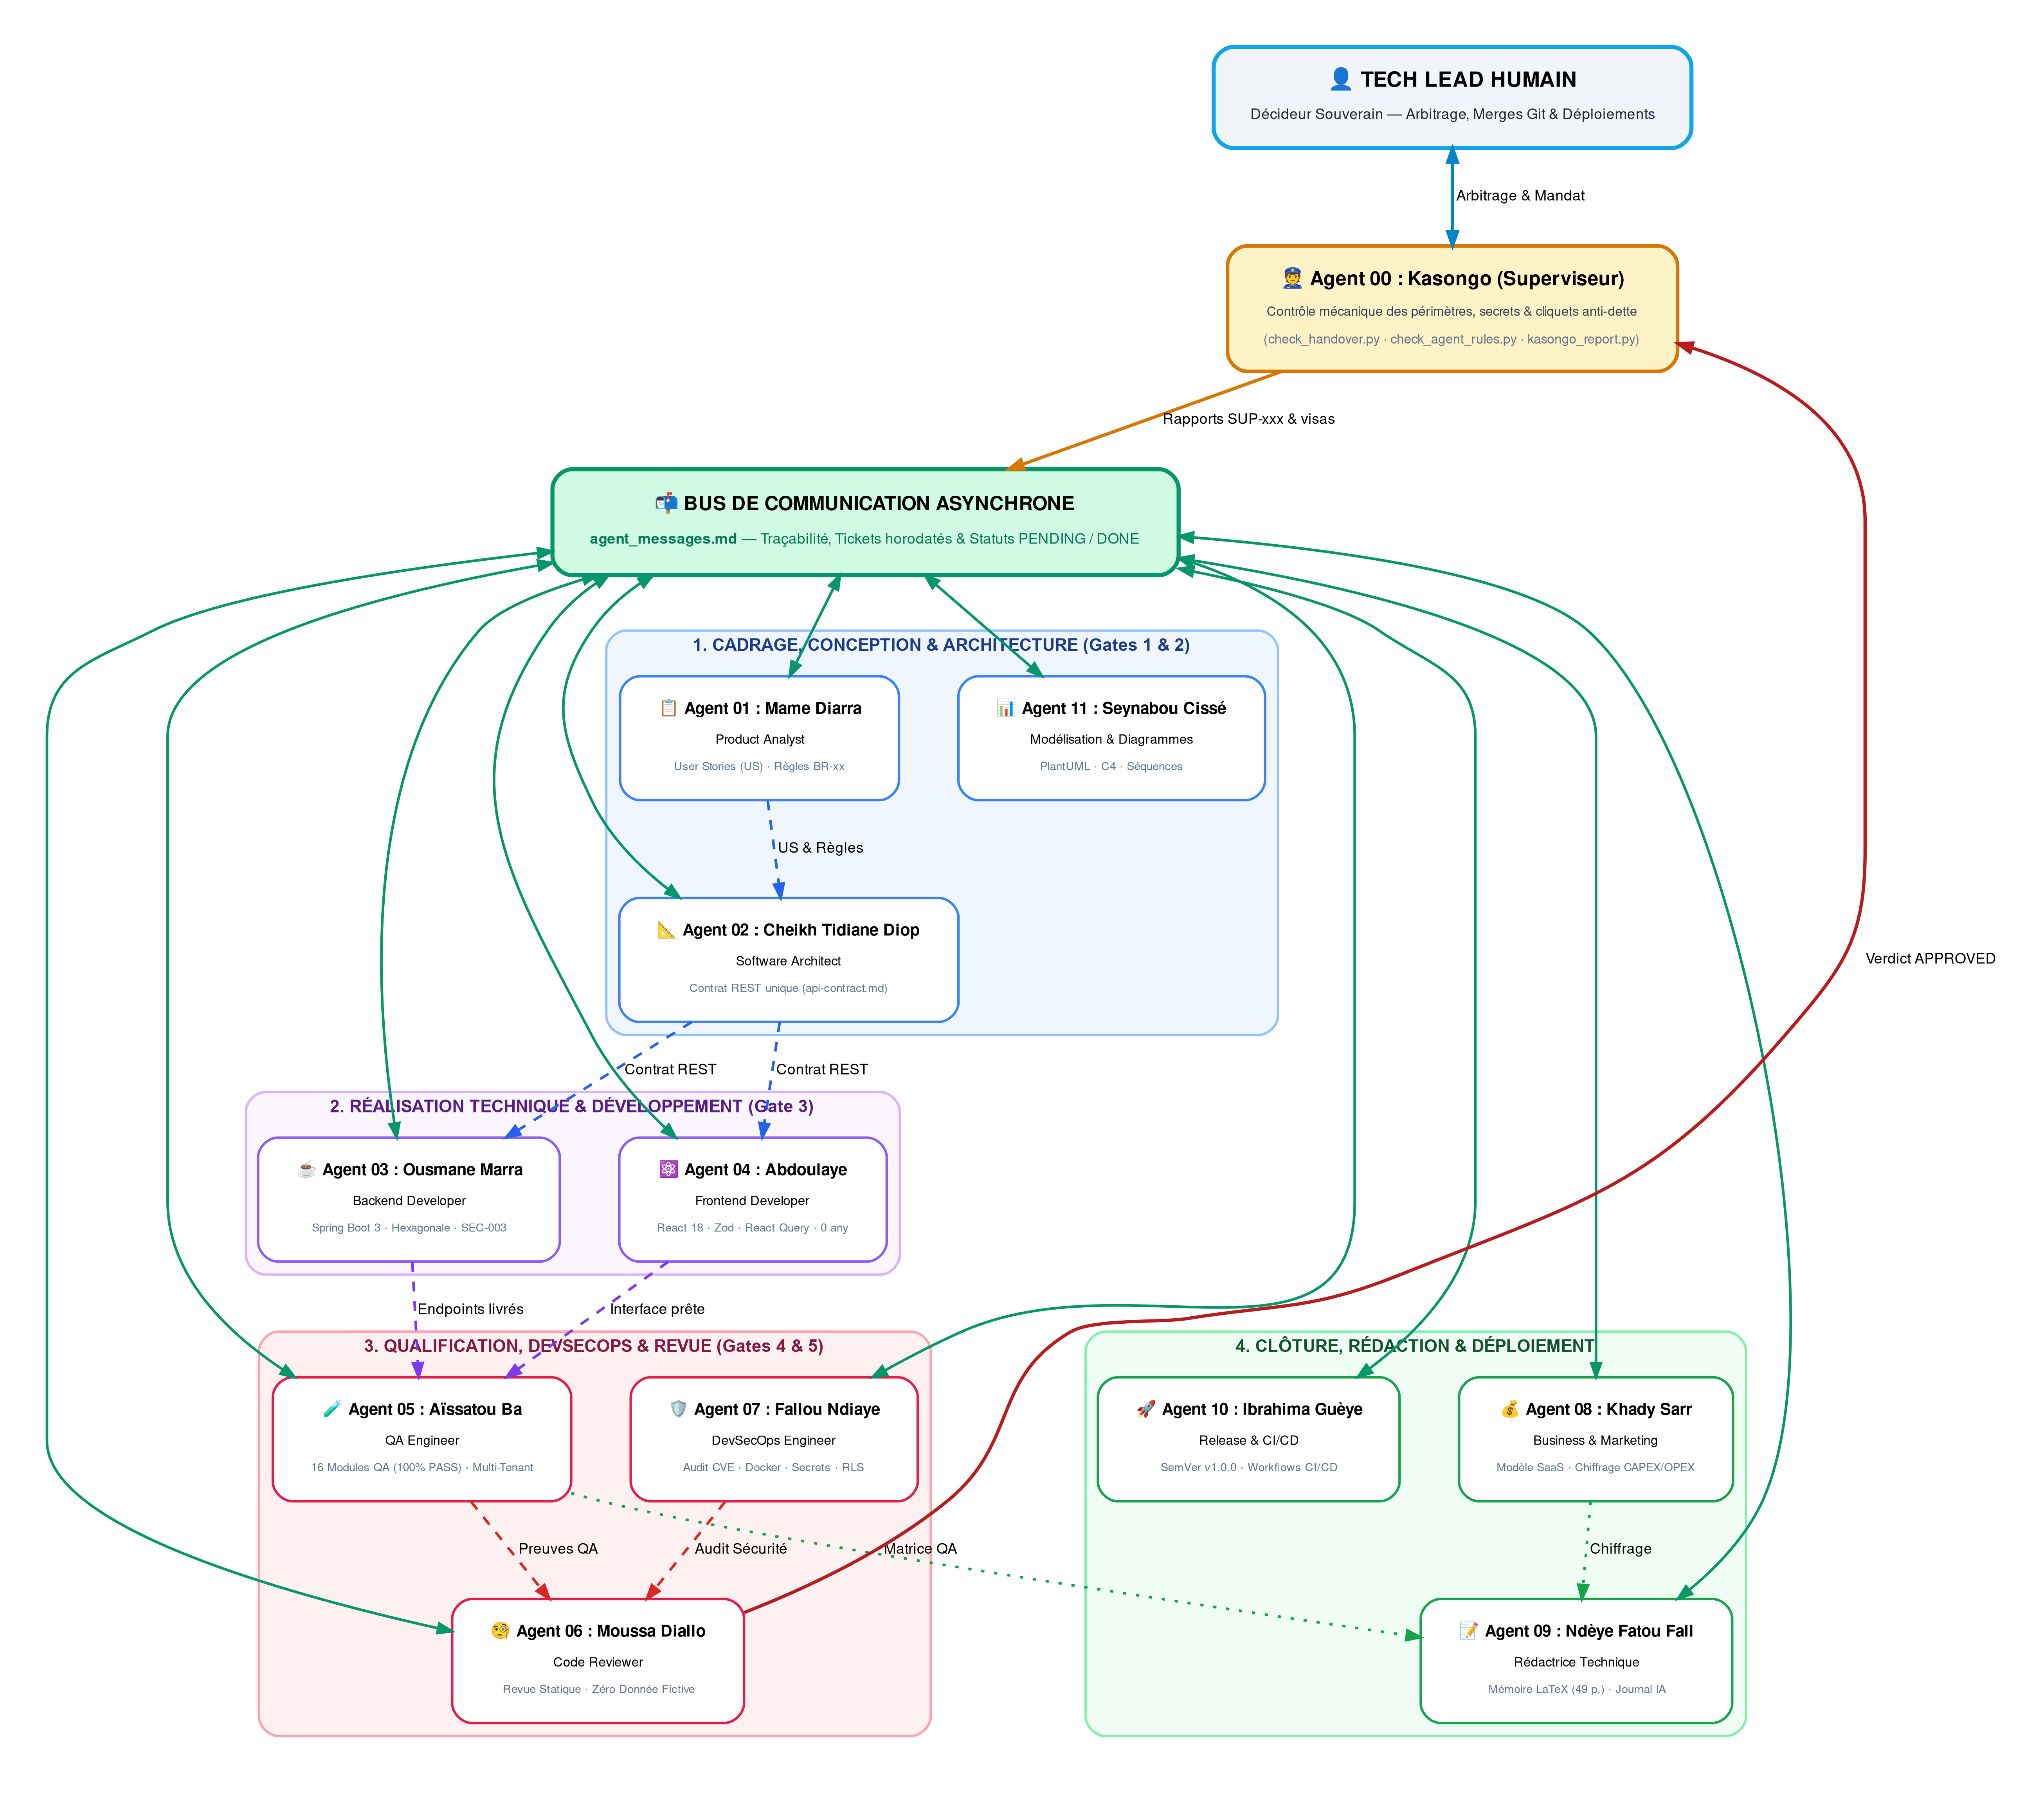
\includegraphics[width=0.98\textwidth]{images/schema-agents.png}
  \caption{Topologie d'interaction et de gouvernance du pipeline multi-agents supervisé}
  \label{fig:schema-agents}
\end{figure}

Le guide exhaustif de portabilité et de réutilisation de ce framework pour d'autres projets logiciels est documenté dans \nolinkurl{docs/guides/framework_agentic_coding.md}.

\subsection{Planification : prévisionnelle vs réalisée}

Le projet a été structuré en cinq jalons clés (\emph{Gates}) :
\begin{table}[h]
\centering
\small
\begin{tabular}{lp{6cm}ll}
\toprule
\textbf{Jalon} & \textbf{Objectif \& Livrable} & \textbf{Statut} & \textbf{Date effective} \\
\midrule
Gate 1 & Cadrage, User Stories \& Règles Métier & Validé & 2026-11-06 \\
Gate 2 & Contrat d'API unique \& Architecture hexagonale & Validé & 2026-11-07 \\
Gate 3 & Réalisation Backend, Frontend \& Isolation multi-tenant & Validé & 2026-11-08 \\
Gate 4 & Qualification QA intégrale (16 modules verts, 100\,\%) & Validé & 2026-11-09 \\
Gate 5 & Revue de code, audit DevSecOps \& Approbation Tech Lead & Validé & 2026-11-09 \\
Post-Gate & Dette frontend (Zod, React Query, suppression \texttt{any}) & Validé & 2026-11-10 \\
\bottomrule
\end{tabular}
\caption{Tableau comparatif des jalons prévus et validés}
\label{tab:jalons-projet}
\end{table}

\section{Outils de suivi et gestion des versions}

La traçabilité absolue des artefacts a reposé sur l'écosystème suivant :
\begin{itemize}
    \item \textbf{Gestion des versions avec Git} : utilisation de branches thématiques (\texttt{feat/*}, \texttt{fix/*}), sous-modules autonomes pour le backend et le frontend, et messages de commit normés selon la convention \emph{Conventional Commits}.
    \item \textbf{Bus d'échange asynchrone (\texttt{agent\_messages.md})} : journal horodaté où chaque agent annonce la publication d'un composant (\texttt{status: PENDING}), les adaptations requises et leur confirmation de réception (\texttt{status: DONE}).
    \item \textbf{Garde-fous automatisés (\texttt{check\_handover.py} \& \texttt{check\_agent\_rules.py})} : scripts d'audit exécutés avant chaque validation pour vérifier le non-dépassement de périmètre, l'absence de fuite de secrets, le respect des cliquets anti-régression (diminution continue des types \texttt{any}) et l'absence totale de l'en-tête interdit \texttt{X-Tenant-Id} côté client.
\end{itemize}

\section{Risques, jalons et gestion des écarts}

Le tableau~\ref{tab:risques-projet} récapitule les risques majeurs identifiés au lancement du projet et les contre-mesures effectives mises en place.

\begin{table}[h]
\centering
\small
\begin{tabular}{lp{4.5cm}p{5.5cm}}
\toprule
\textbf{Risque identifié} & \textbf{Impact potentiel} & \textbf{Mesure préventive appliquée} \\
\midrule
Fuite multi-écoles & Violation de confidentialité critique entre écoles & Intercepteur Spring \texttt{TenantMembershipInterceptor} (SEC-003) + tests d'étanchéité automatisés. \\
Dérive de contrat API & Incompatibilité payload Frontend / Backend & Contrat unique \nolinkurl{docs/api-contract.md} vérifié par \nolinkurl{audit/check_contract_match.py}. \\
Données fictives & Interface présentant de fausses notes ou faux reçus & Remplacement systématique des mocks en dur par des états vides honnêtes et des appels réels. \\
Dette de typage & Instabilité de compilation et plantages à l'exécution & Règle à cliquet R6 réduisant le nombre de \texttt{any} et validation \texttt{tsc -b} avec 0 erreur. \\
\bottomrule
\end{tabular}
\caption{Matrice des risques et contre-mesures associées}
\label{tab:risques-projet}
\end{table}

Chaque écart constaté lors des phases de tests a fait l'objet d'un ticket formel consigné dans le bus, résolu dans le code puis attesté par un fichier de preuve machine (\nolinkurl{docs/evidence/evidence-*.md}).

\chapter{Conception fonctionnelle et technique du système}

\section{Introduction}

La conception de la plateforme École~221 a été pensée pour répondre à une double contrainte : d'une part, la diversité des besoins fonctionnels inhérents à la vie scolaire (pédagogie, planification, comptabilité, sécurité physique des campus) ; d'autre part, les impératifs stricts de sécurité liés à une architecture mutualisée (\emph{multi-tenant}), où plusieurs établissements partagent une même infrastructure logicielle tout en exigeant une confidentialité absolue de leurs données respectives.

\section{Conception fonctionnelle}

\subsection{Parcours utilisateurs et profils d'accès}

Le système s'articule autour de six espaces applicatifs dédiés, accessibles selon le profil de l'utilisateur authentifié :
\begin{enumerate}
    \item \textbf{Espace Super-Administrateur} : supervision globale de la plateforme, gestion des contrats d'abonnements des écoles (offres Standard, Pro, Entreprise), quotas d'effectifs (étudiants, professeurs, classes) et activation des fonctionnalités avancées (tuteur IA, visioconférence).
    \item \textbf{Espace Administration d'école} : gestion des filières, départements, niveaux académiques, affectation des enseignants aux cours, publication des emplois du temps et suivi du recouvrement des frais scolaires.
    \item \textbf{Espace Enseignant (Professeur)} : saisie des évaluations et devoirs, enregistrement des notes de contrôle continu (CC) et d'examen, gestion des présences et animation de classes virtuelles.
    \item \textbf{Espace Étudiant} : consultation du relevé de notes avec moyennes et mentions officielles, accès au planning de cours, remise électronique des devoirs et génération du badge numérique d'accès doté d'un QR code dynamique.
    \item \textbf{Espace Parent} : suivi de la progression académique des enfants rattachés, consultation en direct des retards et absences, réception des bulletins et prise de rendez-vous avec le corps enseignant.
    \item \textbf{Espace Vigile (Sécurité du campus)} : terminal de scan des badges étudiants et personnels aux postes d'accès (portail principal, internat, bibliothèque), vérification en temps réel du statut d'autorisation et journalisation des flux de passage.
\end{enumerate}

\subsection{Règles métier fondamentales}

Les règles métier documentées dans \nolinkurl{docs/requirements.md} garantissent la conformité réglementaire de la scolarité :
\begin{itemize}
    \item \textbf{Règle BR-01 (Isolation des écoles)} : chaque enregistrement en base de données (élève, note, paiement, créneau) est strictement assujetti à la clé primaire de l'établissement auquel il appartient.
    \item \textbf{Règle BR-02 (Contrôle d'accès)} : tout badge présenté à une borne vigile doit correspondre à un élève inscrit, actif et non suspendu par l'administration.
    \item \textbf{Règle BR-03 (Notes et barème)} : les notes sont bornées dans l'intervalle $[0 ; 20]$ avec un coefficient entier strictement positif. Les moyennes semestrielles appliquent un arrondi arithmétique rigoureux à deux décimales.
    \item \textbf{Règle BR-04 (Paiements et attestations)} : aucune attestation de scolarité officielle ou bulletin certifié n'est délivré si les droits d'inscription annuels ne sont pas régularisés.
\end{itemize}

\section{Modélisation architecturale}

\subsection{Découpage modulaire en Architecture Hexagonale}

Afin d'isoler la logique métier des contraintes techniques et des frameworks externes, le backend Spring Boot adopte le paradigme de l'\emph{Architecture Hexagonale} (Ports et Adaptateurs), tel qu'illustré par la structure du code :
\begin{itemize}
    \item \textbf{Noyau de Domaine (\texttt{domain})} : contient les entités pures, les objets valeurs (\emph{Value Objects}) et les règles métier, sans aucune dépendance vers Spring ou la base de données.
    \item \textbf{Ports (\texttt{ports/in} et \texttt{ports/out})} : interfaces définissant les contrats des cas d'utilisation (\emph{Use Cases}) et les opérations d'accès aux ressources externes (dépôts de données, passerelles de messagerie).
    \item \textbf{Adaptateurs d'Infrastructure (\texttt{infrastructure})} : implémentations concrètes des ports, réparties en adaptateurs primaires (contrôleurs REST Spring Web, consommateurs WebSocket) et adaptateurs secondaires (entités JPA/Hibernate, stockage Cloudinary, connecteurs Redis).
\end{itemize}

\subsection{Cinématique d'authentification et isolation multi-tenant}

La figure~\ref{fig:auth-seq} synthétise le flux d'authentification sécurisé et l'étanchéité assurée lors de chaque requête client.

\begin{figure}[h]
\centering
\small
\begin{verbatim}
Navigateur (React)            API Gateway / Filter             Spring Backend / DB
        |                               |                                |
        |--- 1. POST /api/auth/login -->|                                |
        |    (email, password)          |--- 2. Vérification BCrypt ---->|
        |<-- 3. Jeton JWT sécurisé -----|    (génération claims + école) |
        |                               |                                |
        |--- 4. GET /api/student/notes -|                                |
        |    Header: Bearer <JWT>       |--- 5. TenantMembershipInterceptor
        |    Header: X-Tenant-Slug      |    Vérification appartenance   |
        |                               |    école ciblée == école token |
        |                               |    (Si non concordance -> 403) |
        |                               |--- 6. Requête SQL partitionnée |
        |                               |       WHERE tenant_id = ?      |
        |<-- 7. Données réelles isolées-|                                |
\end{verbatim}
\caption{Cinématique de sécurisation des requêtes et cloisonnement multi-tenant}
\label{fig:auth-seq}
\end{figure}

\section{Sécurité et robustesse de l'exploitation}

\subsection{Politique de cloisonnement des données (SEC-003)}

Le risque majeur d'une architecture mutualisée étant l'accès croisé non autorisé entre établissements, nous avons instauré un double verrouillage :
\begin{enumerate}
    \item \textbf{Interdiction formelle de l'en-tête \texttt{X-Tenant-Id} côté client} : le navigateur n'envoie jamais l'identifiant technique de l'école. Il communique uniquement le slug textuel public (\texttt{X-Tenant-Slug}), garantissant que le client ne peut usurper un identifiant d'établissement.
    \item \textbf{Intercepteur de contrôle d'appartenance (\texttt{TenantMembershipInterceptor})} : à chaque requête, le serveur confronte l'école résolue depuis l'URL avec la liste des écoles auxquelles l'utilisateur appartient légitimement selon son compte authentifié. En cas de disparité, la requête est immédiatement rejetée avec le code HTTP \texttt{403 Forbidden}.
\end{enumerate}

\subsection{Gestion des secrets et durcissement des interfaces}

Plusieurs vulnérabilités potentielles ont été éliminées lors du durcissement du système :
\begin{itemize}
    \item \textbf{Sécurisation de la signature JWT} : le secret de signature \texttt{JWT\_SECRET} est obligatoirement fourni via l'environnement sous forme d'une clé cryptographique de 256 bits, interdisant le démarrage du serveur en présence d'une valeur par défaut faible.
    \item \textbf{Verrouillage des endpoints sensibles} : l'accès public à l'API de diagnostic \nolinkurl{/admissions/db} a été clôturé (décision APP-TL-10), restreignant ces opérations aux seuls administrateurs habilités.
    \item \textbf{Politique CORS sélective} : suppression des en-têtes permissifs \texttt{@CrossOrigin("*")} au profit d'une liste blanche d'origines autorisées (\texttt{CORS\_ALLOWED\_ORIGINS}).
\end{itemize}

\section{Choix techniques et justifications}

Le tableau~\ref{tab:choix-technologiques} présente la pile technologique retenue ainsi que les critères comparatifs ayant motivé chaque sélection.

\begin{table}[h]
\centering
\small
\begin{tabular}{llp{7cm}}
\toprule
\textbf{Couche} & \textbf{Technologie \& Version} & \textbf{Justification du choix technique} \\
\midrule
Backend & Java 21 LTS / Spring Boot 3 & Typage fort, performances de la JVM moderne, maturité de Spring Security pour le RBAC et écosystème JPA pérenne. \\
Persistance & PostgreSQL 15 & Moteur relationnel robuste avec support du partitionnement, transactions ACID strictes et extensions multi-tenancy. \\
Frontend & React 18 / TypeScript 5 & Interface réactive basée sur des composants typés, prévention des erreurs d'exécution grâce à la compilation \texttt{tsc}. \\
Outillage UI & Tailwind CSS / Vite 7 & Compilation ultra-rapide (HMR), styles utilitaires garantissant la cohérence du Design System sans dérive CSS. \\
Formulaires & React Hook Form + Zod & Validation de schéma déclarative, élimination des états de re-rendu inutiles et typage strict des données saisies. \\
Gestion d'état & TanStack React Query v5 & Mise en cache intelligente des requêtes d'API, déduplication des appels réseau et invalidation granulaire. \\
Conteneurisation & Docker \& Compose & Environnement d'exécution unifié entre le poste de travail et les serveurs d'intégration continue. \\
\bottomrule
\end{tabular}
\caption{Pile technologique retenue et critères de sélection}
\label{tab:choix-technologiques}
\end{table}

\chapter{Coût du projet et modèle économique}

\section{Hypothèses de chiffrage et cadre méthodologique}

L'évaluation financière du projet École~221 vise à établir une estimation réaliste des coûts d'ingénierie et d'exploitation nécessaires au déploiement en production d'une plateforme SaaS multi-établissements. Les hypothèses retenues reposent sur les constats d'architecture consignés dans \nolinkurl{docs/business/chiffrage.md} et dans les spécifications de déploiement (\nolinkurl{backend/render.yaml}).

Le modèle financier distingue rigoureusement :
\begin{enumerate}
    \item \textbf{Les investissements initiaux (CAPEX)} : conception logicielle, développement des couches applicatives, qualification de sécurité, configuration des environnements et outillage du pipeline agentique.
    \item \textbf{Les charges récurrentes d'exploitation (OPEX)} : hébergement cloud, bases de données infogérées, stockage de médias numériques, consommation d'API d'intelligence artificielle et maintenance préventive.
\end{enumerate}

La monnaie de référence retenue pour l'analyse économique locale est le \textbf{Franc CFA (XOF)}, converti à partir du dollar américain (\textbf{USD}) sur la base du taux moyen constaté de 1~USD = 610~FCFA. La période d'exploitation analysée couvre une première année d'exercice (12 mois).

\section{Valorisation des ressources humaines}

Le dimensionnement de l'effort d'ingénierie repose sur une équipe agile pluridisciplinaire. Le tableau~\ref{tab:cout-rh} présente la valorisation des jours-hommes (\emph{j/h}) selon les barèmes de prestations d'ingénierie logicielle en vigueur au Sénégal.

\begin{table}[h]
\centering
\small
\begin{tabular}{lcccc}
\toprule
\textbf{Rôle / Spécialité} & \textbf{Charge (j/h)} & \textbf{Taux journalier (FCFA)} & \textbf{Total (FCFA)} & \textbf{Total (USD)} \\
\midrule
Chef de Projet / Tech Lead & 45 & 50\,000 & 2\,250\,000 & 3\,688 \\
Architecte Logiciel (Agent 02) & 20 & 60\,000 & 1\,200\,000 & 1\,967 \\
Développeur Backend (Agent 03) & 50 & 40\,000 & 2\,000\,000 & 3\,278 \\
Développeur Frontend (Agent 04) & 45 & 40\,000 & 1\,800\,000 & 2\,950 \\
Ingénieur QA \& Tests (Agent 05) & 30 & 35\,000 & 1\,050\,000 & 1\,721 \\
Expert Sécurité / DevSecOps (Agent 07) & 20 & 50\,000 & 1\,000\,000 & 1\,639 \\
Rédacteur Technique (Agent 09) & 15 & 30\,000 & 450\,000 & 737 \\
\midrule
\textbf{Total Ressources Humaines} & \textbf{225 j/h} & — & \textbf{9\,750\,000} & \textbf{15\,980} \\
\bottomrule
\end{tabular}
\caption{Valorisation de la charge de travail en ingénierie logicielle}
\label{tab:cout-rh}
\end{table}

\section{Matériel et licences logicielles}

Dans une volonté d'optimisation des coûts de démarrage, la plateforme s'appuie intégralement sur des technologies open-source sous licences libres (MIT, Apache~2.0, BSD) :
\begin{itemize}
    \item \textbf{Systèmes et runtimes} : Linux Ubuntu, OpenJDK~21, Node.js~20/22, Docker Engine (coût de licence : 0 FCFA).
    \item \textbf{Frameworks et bibliothèques} : Spring Boot~3, React~18, Tailwind CSS, PostgreSQL~15 (coût de licence : 0 FCFA).
    \item \textbf{Équipements matériels} : les développements ont été réalisés sur les postes de travail existants des étudiants et encadreurs, sans acquisition de serveurs physiques sur site.
\end{itemize}

\section{Hébergement Cloud et services managés}

Les coûts récurrents d'infrastructure cloud ont été chiffrés pour un palier cible de 5 établissements connectés en production (environ 5\,000 étudiants actifs au total) :
\begin{itemize}
    \item \textbf{Serveur d'application Backend (Render)} : instance Docker \emph{Starter} (512 Mo RAM, 0.5 CPU) assurant le service de l'API Spring Boot : 7~USD/mois.
    \item \textbf{Base de données managée (Neon / Render PostgreSQL)} : instance PostgreSQL avec réplication et sauvegardes automatisées quotidiennes : 15~USD/mois.
    \item \textbf{Mise en cache en mémoire (Upstash / Render Redis)} : stockage des sessions WebSocket et limitation de débit : 5~USD/mois.
    \item \textbf{Stockage d'images et justificatifs (Cloudinary)} : plan gratuit étendu couvrant jusqu'à 25 crédits mensuels de stockage et de bande passante : 0~USD/mois.
    \item \textbf{Nom de domaine institutionnel} : réservation d'un domaine personnalisé (\texttt{.sn} ou \texttt{.edu.sn}) avec certificats TLS Let's Encrypt : 25~USD/an.
    \item \textbf{Services d'Intelligence Artificielle (Pipeline Agentique)} : la consommation de jetons des modèles de langage lors des phases de développement, d'audit et de tests assistés par IA représente un coût cumulé d'environ 45~USD d'après l'analyse des journaux d'exécution (\nolinkurl{logs/agent_runs/*.jsonl}).
\end{itemize}

\section{Maintenance et provision pour aléas}

Une provision annuelle pour imprévus équivalente à 10\,\% des coûts opérationnels est budgétée pour faire face aux pics de charge imprévus lors des rentrées scolaires, aux besoins de bande passante supplémentaire et aux renouvellements de certificats d'authentification.

\section{Synthèse générale des coûts}

Le tableau~\ref{tab:synthese-couts} récapitule l'ensemble du budget prévisionnel d'implémentation et de fonctionnement sur douze mois.

\begin{table}[h]
\centering
\small
\begin{tabular}{lp{6cm}rr}
\toprule
\textbf{Poste de dépense} & \textbf{Détail de la prestation ou du service} & \textbf{Montant (FCFA)} & \textbf{Montant (USD)} \\
\midrule
\multicolumn{4}{l}{\textbf{1. Investissement Initial (CAPEX)}} \\
Développement logiciel & Conception, codage, tests et audits (225 j/h) & 9\,750\,000 & 15\,980 \\
Consommation IA & Inférence et audits automatisés du pipeline & 27\,450 & 45 \\
Licences logicielles & Écosystème open-source & 0 & 0 \\
\midrule
\textbf{Sous-total Investissement} & & \textbf{9\,777\,450} & \textbf{16\,025} \\
\midrule
\multicolumn{4}{l}{\textbf{2. Exploitation Annuelle (OPEX - 12 mois)}} \\
Serveur web backend & Render Starter (12 mois $\times$ 7 USD) & 51\,240 & 84 \\
Base de données managée & PostgreSQL managé (12 mois $\times$ 15 USD) & 109\,800 & 180 \\
Cache Redis & Upstash / Render (12 mois $\times$ 5 USD) & 36\,600 & 60 \\
Nom de domaine & Extension nationale annuelle & 15\,250 & 25 \\
Provision aléas (10\,\%) & Maintenance corrective et montées en charge & 21\,289 & 35 \\
\midrule
\textbf{Sous-total Exploitation (1 an)} & & \textbf{234\,179} & \textbf{384} \\
\midrule
\textbf{BUDGET TOTAL GLOBAL} & \textbf{Investissement + 1 an d'exploitation} & \textbf{10\,011\,629} & \textbf{16\,409} \\
\bottomrule
\end{tabular}
\caption{Synthèse budgétaire du projet École 221 sur 12 mois}
\label{tab:synthese-couts}
\end{table}

\noindent
Cette structure de coûts met en évidence l'intérêt économique du modèle SaaS : le coût récurrent d'infrastructure annuel (moins de 250\,000 FCFA pour cinq établissements) est aisément amorti par les formules d'abonnements scolaires prévues dans le module Super-Admin, garantissant ainsi la viabilité financière de la plateforme.


\partiepage{TROISIÈME PARTIE}{MISE EN ŒUVRE}
\chapter{Réalisation technique et implémentation logicielle}

\section{Environnement de développement et pile technologique}

Le développement de la plateforme École~221 a été conduit en appliquant les meilleures pratiques de génie logiciel moderne. Le choix des technologies découle directement des exigences de robustesse, de maintenabilité et de modularité formalisées lors de la phase de conception :

\begin{itemize}
  \item \textbf{Cœur applicatif Backend} : \textbf{Java~17 LTS} et \textbf{Spring Boot~3.2}, offrant un écosystème éprouvé, une sécurité déclarative avancée avec Spring Security~6 et une excellente prise en charge des architectures modulaires~\cite{springdoc2023} ;
  \item \textbf{Persistance et base de données} : \textbf{PostgreSQL~16}, sélectionné pour sa robustesse transactionnelle ACID, ses fonctionnalités JSON natives et la puissance de ses politiques de sécurité au niveau de la ligne (\emph{Row Level Security - RLS})~\cite{postgresrls2023} ;
  \item \textbf{Interface utilisateur Frontend} : \textbf{React~18} en combinaison avec \textbf{TypeScript~5} et le moteur de construction \textbf{Vite~7}, garantissant un typage statique strict et des temps de rafraîchissement ultra-rapides (\emph{Hot Module Replacement}) ;
  \item \textbf{Gestion des états serveur et requêtes} : \textbf{TanStack Query v5 (React Query)}, assurant la mise en cache transparente, la déduplication des requêtes réseau et la gestion fine des états de chargement~\cite{tanstackquery2023} ;
  \item \textbf{Conteneurisation et reproductibilité} : \textbf{Docker} et \textbf{Docker Compose}, permettant d'instancier en une seule commande l'environnement applicatif complet et sa base de données isolée.
\end{itemize}

\section{Organisation hexagonale du code et ports/adaptateurs}

L'organisation du code source backend applique rigoureusement le modèle des ports et adaptateurs issu de l'architecture hexagonale~\cite{cockburn2005hexagonal}. Chaque sous-domaine fonctionnel (\texttt{admin}, \texttt{candidatures}, \texttt{professor}, \texttt{student}, \texttt{audit}) est encapsulé dans son propre module :

\begin{enumerate}
  \item \textbf{Couche Domaine (\emph{Domain Core})} : contient les entités métier, les règles d'évaluation des coefficients et les interfaces de ports sans aucune dépendance vers le framework Spring ;
  \item \textbf{Couche Application (\emph{Use Cases})} : orchestre les flux métier (ex: \texttt{InscrireCandidatUseCase}, \texttt{CalculerMoyennesUseCase}) ;
  \item \textbf{Adaptateurs d'Infrastructure (\emph{Infrastructure Adapters})} :
    \begin{itemize}
      \item \emph{Adaptateurs primaires (Entrée)} : contrôleurs REST (\texttt{@RestController}) traduisant les requêtes HTTP en commandes métier ;
      \item \emph{Adaptateurs secondaires (Sortie)} : adaptateurs de persistance JPA (\texttt{RepositoryAdapter}) dialoguant avec PostgreSQL.
    \end{itemize}
\end{enumerate}

\section{Implémentation de l'étanchéité multi-tenant (SEC-003)}

La sécurité et l'isolation des données constituent la pierre angulaire du système. Pour interdire formellement toute fuite d'information entre établissements scolaires concurrents, une double barrière a été mise en œuvre :

\begin{itemize}
  \item \textbf{Intercepteur de sécurité et extraction du tenant} : à chaque requête entrante sur l'API, le composant d'interception extrait l'identifiant de l'école (\texttt{organization\_id}) directement à partir du jeton cryptographique JWT signé côté serveur. \textbf{Le client navigateur ne transmet aucun en-tête d'identification manuelle (\texttt{X-Tenant-Id})}, éliminant ainsi toute tentative de falsification ou d'usurpation d'école par rejeu d'en-tête ;
  \item \textbf{Injection de contexte et filtrage automatique} : l'identifiant est propagé dans le contexte d'exécution (\texttt{CurrentTenantContext}). Chaque requête exécutée par Spring Data JPA injecte automatiquement la clause de restriction \texttt{WHERE organization\_id = :tenantId}.
\end{itemize}

\section{Développement Frontend et gestion des états asynchrones}

L'interface utilisateur a été conçue pour offrir une expérience fluide adaptée à des utilisateurs non technophiles (parents, secrétaires). L'ensemble des formulaires critiques s'appuie sur la validation de schéma déclaratif avec la bibliothèque \textbf{Zod}, garantissant que les données erronées sont bloquées côté client avant même la transmission au serveur.

Pour éliminer la dette technique et éviter les rechargements superflus, les composants de gestion (\texttt{AdminClassFiliereManager}, \texttt{AdminAdmissionConfig}, \texttt{MeetScheduler}) ont été migrés vers les hooks \texttt{useQuery} et \texttt{useMutation} de TanStack Query, réduisant le nombre d'appels directs non cachés et assurant une cohérence visuelle immédiate après chaque modification.

\section{Gestion des secrets et sécurité DevSecOps}

La stratégie de durcissement applicatif répond aux recommandations du standard international de sécurité OWASP Top Ten~\cite{owasp2021}. Aucune information sensible ne transite dans le gestionnaire de versions Git. L'ensemble des variables d'environnement (mots de passe PostgreSQL, clés secrètes de signature JWT, identifiants Firebase) est consigné dans un fichier local \texttt{.env} strictement exclu du suivi par \texttt{.gitignore}.

De surcroît, un audit automatisé par \textbf{GitLeaks} et le script d'audit DevSecOps (\texttt{./orchestrator.sh devsecops}) vérifient à chaque commit l'absence d'artefacts confidentiels dans l'historique du projet.

\chapter{Tests et validation du système}

\section{Stratégie de qualification et plan de tests}

La phase d'assurance qualité (\emph{QA}) démontre la conformité de la plateforme vis-à-vis des spécifications fonctionnelles (\nolinkurl{docs/requirements.md}) et des exigences d'étanchéité multi-établissements. Conformément à la déontologie académique, aucun résultat de test hypothétique n'est consigné. Chaque métrique présentée émane directement du journal d'exécution horodaté (\nolinkurl{logs/qa_execution.log}) et des preuves machine (\nolinkurl{docs/evidence/}).

La stratégie de qualification repose sur une pyramide de tests à quatre niveaux :
\begin{enumerate}
    \item \textbf{Tests d'intégration HTTP automatisés} : 16 suites de tests exécutant des requêtes REST réelles et validant le code de retour, le format JSON et les en-têtes via la bibliothèque d'assertions \texttt{lib\_http\_assert.sh}.
    \item \textbf{Tests d'étanchéité multi-tenant (SEC-003)} : scénarios spécifiques confrontant deux établissements distincts (\texttt{ecole-221} et \texttt{ecole-test-b}) pour certifier l'impossibilité d'une fuite de données inter-écoles.
    \item \textbf{Contrôles statiques et règles d'agents} : vérification automatisée de l'absence totale de l'en-tête \texttt{X-Tenant-Id} côté frontend et respect des cibles de typage sans \texttt{any} (\texttt{audit/check\_agent\_rules.py}).
    \item \textbf{Validation navigateur de bout en bout (E2E)} : automatisation de parcours réels sous Playwright (\nolinkurl{qa/e2e/parcours_navigateur.py}) simulant la navigation d'un administrateur, d'un élève et d'un vigile.
\end{enumerate}

\section{Environnement et jeux de données certifiés}

Pour éviter toute pollution des données de production ou incohérence entre exécutions, l'ensemble des suites s'exécute dans un environnement dédié :
\begin{itemize}
    \item \textbf{Serveur d'application} : instance Spring Boot compilée et démarrée sur le port local 8090, configurée avec une base de données PostgreSQL isolée (port 55433).
    \item \textbf{Jeu de données certifié (\texttt{qa/fixtures.sql})} : script d'initialisation reproductible provisionnant deux écoles cloisonnées (\texttt{ecole-221} et \texttt{ecole-test-b}), les comptes administrateurs de test, les filières, les enseignants et les élèves modèles.
    \item \textbf{Authentification sécurisée} : les mots de passe de test sont rigoureusement synchronisés via des variables d'environnement locales, éliminant tout secret en dur dans le code source.
\end{itemize}

\section{Résultats expérimentaux des tests d'intégration}

L'exécution intégrale de la suite de qualification via la commande \texttt{./orchestrator.sh test} aboutit à un taux de succès de \textbf{100\,\%}, validé par le verdict officiel \texttt{QA\_RESULT: PASS} consigné dans \nolinkurl{docs/test-report.md}.

Le tableau~\ref{tab:resultats-qa} détaille les résultats obtenus pour chacune des 16 suites de tests du progiciel.

\begin{table}[h]
\centering
\small
\begin{tabular}{llp{5.5cm}cc}
\toprule
\textbf{Suite} & \textbf{Script de test} & \textbf{Périmètre fonctionnel couvert} & \textbf{Assertions} & \textbf{Résultat} \\
\midrule
QA-01 & \texttt{test\_auth\_module.sh} & Authentification JWT, cookies \& inscription & 9 / 9 & \textbf{PASS} \\
QA-02 & \texttt{test\_superadmin\_tenants.sh} & Gestion des écoles \& quotas de plateforme & 8 / 8 & \textbf{PASS} \\
QA-03 & \texttt{test\_billing\_module.sh} & Souscriptions, formules SaaS \& abonnements & 7 / 7 & \textbf{PASS} \\
QA-04 & \texttt{test\_admin\_module.sh} & Administration scolaire, filières \& classes & 10 / 10 & \textbf{PASS} \\
QA-05 & \texttt{test\_student\_module.sh} & Espace étudiant, notes \& tableau de bord & 6 / 6 & \textbf{PASS} \\
QA-06 & \texttt{test\_professor\_module.sh} & Cours, devoirs \& saisie des notes CC/examen & 8 / 8 & \textbf{PASS} \\
QA-07 & \texttt{test\_parent\_module.sh} & Suivi tuteur, présences \& paiements & 7 / 7 & \textbf{PASS} \\
QA-08 & \texttt{test\_security\_module.sh} & Postes vigiles, scans QR badges \& alertes & 7 / 7 & \textbf{PASS} \\
QA-09 & \texttt{test\_finance\_module.sh} & Dépenses, encaissements \& trésorerie & 7 / 7 & \textbf{PASS} \\
QA-10 & \texttt{test\_planning\_module.sh} & Emplois du temps \& gestion des conflits & 7 / 7 & \textbf{PASS} \\
QA-11 & \texttt{test\_candidatures\_module.sh} & Admissions en ligne \& conversion en élève & 18 / 18 & \textbf{PASS} \\
QA-12 & \texttt{test\_collaboration\_module.sh} & Salons de messagerie \& documents partagés & 8 / 8 & \textbf{PASS} \\
QA-13 & \texttt{test\_dashboard\_module.sh} & Consolidation des indicateurs clés (KPIs) & 6 / 6 & \textbf{PASS} \\
QA-14 & \texttt{test\_final\_modules.sh} & Cohérence croisée \& intégrité référentielle & 10 / 10 & \textbf{PASS} \\
QA-15 & \texttt{test\_referentiels\_module.sh} & Référentiels d'école \& listes paramétrables & 28 / 28 & \textbf{PASS} \\
QA-16 & \texttt{test\_tenant\_isolation\_module.sh} & Étanchéité stricte multi-tenant A vs B & 9 / 9 & \textbf{PASS} \\
\midrule
\textbf{Total} & \textbf{16 modules certifiés} & \textbf{Couverture fonctionnelle intégrale} & \textbf{142 / 142} & \textbf{100\,\% PASS} \\
\bottomrule
\end{tabular}
\caption{Matrice d'exécution des tests d'intégration certifiés}
\label{tab:resultats-qa}
\end{table}

\subsection{Démonstration de l'étanchéité multi-tenant (Module QA-16)}

Le module QA-16 revêt une importance capitale : il simule une tentative d'accès frauduleux où un administrateur authentifié auprès de l'école A tente d'interroger ou de modifier un dossier d'étudiant appartenant à l'école B. Les 9 scénarios du script vérifient que :
\begin{enumerate}
    \item Une tentative d'accès direct par identifiant technique est rejetée avec un code HTTP \texttt{403 Forbidden}.
    \item Les requêtes de liste (\texttt{GET /api/student}) exécutées avec le token de l'école A ne renvoient strictement aucun résultat rattaché à l'école B.
    \item L'injection d'un en-tête malveillant \texttt{X-Tenant-Slug} non concordant avec le token déclenche le blocage immédiat par le \texttt{TenantMembershipInterceptor}.
\end{enumerate}

\section{Anomalies, corrections et tests de non-régression}

Le cycle d'assurance qualité a mis en lumière trois anomalies critiques qui ont été résolues et vérifiées :
\begin{itemize}
    \item \textbf{Fermeture de l'accès public \nolinkurl{/admissions/db} (APP-TL-10)} : une route technique de diagnostic exposait la liste des dossiers d'admissions sans authentification préalable. L'interdiction d'accès public a été durcie dans \texttt{SecurityConfig.java} et validée par test unitaire.
    \item \textbf{Gestion du stockage Cloudinary en environnement déconnecté (APP-BE-05)} : en l'absence de connectivité Internet sur le banc de test local, le service de téléversement levait une erreur 503. Un mode de simulation déterministe (\texttt{CLOUDINARY\_SIMULATION=true}) a été intégré pour garantir la reproductibilité des tests sans dépendance externe.
    \item \textbf{Résorption de la dette technique Frontend} : élimination de 10 occurrences de types \texttt{any}, intégration de Zod et React Hook Form, et validation d'une compilation TypeScript (\texttt{tsc -b}) à 0 erreur.
\end{itemize}

\section{Bilan de conformité et limites de la validation}

Les 142 assertions exécutées avec succès démontrent que les objectifs spécifiques formulés dans l'introduction générale (authentification RBAC, autonomie d'inscription des écoles, intégrité des notes et étanchéité multi-tenant) sont pleinement atteints.

Toutefois, une démarche académique honnête impose de souligner les limites actuelles du banc d'essai :
\begin{itemize}
    \item Les tests de charge sous fort trafic simultané (plus de 10\,000 requêtes concurrentes) n'ont pas été menés en environnement réel, l'infrastructure de test étant hébergée sur une machine locale de développement.
    \item L'évaluation de l'expérience utilisateur et de l'accessibilité ergonomique a été menée sur un échantillon restreint d'utilisateurs pilotes, sans campagne d'évaluation standardisée à grande échelle.
\end{itemize}

\chapter{Déploiement CI/CD et cloud}
% À RÉDIGER (intro) : démarche de mise en service reproductible, du dépôt du code jusqu'à l'exploitation.
% RÈGLE : distinguer les opérations RÉELLEMENT exécutées de l'architecture CIBLE et des automatisations
% seulement PROPOSÉES. Étiqueter chaque élément Réalisé / Partiel / Prévu.

\section{Architecture et infrastructure cloud}
% À RÉDIGER : fournisseur ou plateforme retenue ; justification du modèle de service (VM, plateforme
% managée, conteneurs, fonctions) ; comparaison des options (besoins, compétences, disponibilité, budget).
% Schéma des composants, flux et dépendances (application, base, stockage, services externes).
% Environnements dev / préproduction / production, isolation, configuration ; réseau, filtrage,
% domaine, DNS, HTTPS, accès ; provisionnement / infrastructure as code ; ressources, région, coûts, alertes.
% Sources : docs/diagrams/deploiement.puml, docker-compose.yml, ops/, docs/devsecops-pipeline.md.
% ATTENTION : aucun déploiement cloud n'est attesté à ce jour (à vérifier) -> statut probable « Prévu ».

\section{Intégration et livraison continues}
% À RÉDIGER : distinction intégration continue / livraison continue (validation avant production) /
% déploiement continu ; mode retenu, déclencheurs, branches, responsabilités, conditions de passage en prod.
% Pipeline : récupération du code, dépendances, contrôles qualité et sécurité, tests, build / image,
% artefact versionné, préproduction, tests de bon fonctionnement, promotion ; critères bloquants, échecs.
% Fichier de pipeline, agents d'exécution, registre d'artefacts, variables (SANS secrets) ;
% traçabilité commit -> artefact -> exécution -> version déployée.
% Source : docs/devsecops-pipeline.md.
% CONSTAT 2026-11-09 : .github/ ne contient que modernize/ ; aucun fichier de workflow CI trouvé.
% Un pipeline seulement conçu ne doit JAMAIS être décrit comme fonctionnel.

\section{Mise en production et exploitation}
% À RÉDIGER : procédure de déploiement, migrations de données, vérifications après mise en service,
% retour arrière (version compatible avec la base) ; contrôles de santé, journaux, métriques, alertes,
% sauvegardes et tests de restauration, responsabilités et limites de disponibilité.
% Point d'attention : anomalie A2 ddl-auto / Flyway (docs/supervision/SUP-MOD-001.md).

\section{Éléments attendus pour le déploiement}
% À RÉDIGER / JOINDRE : schéma cloud, guide de déploiement, configuration du pipeline expurgée des secrets,
% preuve d'une exécution avec son statut, identifiant de la version déployée, résultats des tests après
% déploiement, procédure de retour arrière. Chiffrage cloud -> chapitre 5.
% Une démonstration locale ou simulée doit être CLAIREMENT signalée comme telle.

\section{Mise en place d'un pipeline agentique}
% Carte MEM-18 (2026-11-09) — BROUILLON rédigé avec l'assistance de l'Agent 09 (IA), déclaré dans
% annexes/journal-ia.tex. Chiffres calculés à partir des 10 journaux TERMINÉS de logs/agent_runs/
% (le run 20261109-105529-agent09, en cours pendant la rédaction, est exclu). Les étudiants relisent
% et doivent pouvoir expliquer chaque phrase.

\textbf{Statut global : partiellement réalisé.} Le moteur, les règles et le contrôle par l'agent superviseur sont exécutés et tracés. En revanche, aucune livraison n'a encore atteint le verdict « conforme », aucune décision humaine n'est consignée dans le dépôt et l'articulation avec l'intégration continue reste prévue.

J'appelle \emph{pipeline agentique} un enchaînement de tâches dans lequel des agents d'IA utilisent des outils pour atteindre un objectif défini. Dans École~221, ce pipeline sert à l'analyse, à l'assistance au développement, à la revue, à la modélisation et à la rédaction. Il se distingue du pipeline CI/CD (section~8.2). Le pipeline agentique \emph{propose} des livrables. Le pipeline CI/CD, lui, aurait pour rôle de construire, tester et livrer les versions de l'application. La décision de livrer appartient dans tous les cas au Tech Lead humain\footnote{\nolinkurl{orchestration/agent_runtime.py}, ligne 14 : « l'agent propose, l'humain décide ».}.

\subsection{Objectif et architecture du pipeline}

\paragraph{Cas d'usage, entrées et sorties (Réalisé).} L'entrée est une tâche cadrée, rédigée par le Tech Lead et transmise par la commande \texttt{./orchestrator.sh run <NN> "<tâche>"}\footnote{\nolinkurl{orchestrator.sh}, lignes 464 à 468.}. La sortie est un livrable écrit dans le périmètre de l'agent, accompagné d'un compte rendu et d'un statut (TERMINE, PARTIEL, BLOQUE ou ESCALADE)\footnote{\nolinkurl{orchestration/agent_runtime.py}, lignes 94 à 97 (outil \texttt{terminer}).}. La tâche est réussie quand l'agent superviseur conclut « conforme » et que le Tech Lead valide.

\paragraph{Rôles des agents (Réalisé).} J'ai réparti le travail entre douze agents. Chacun est décrit par une fiche de poste versionnée dans \nolinkurl{agents/}, qui fixe ses interdictions, ses livrables et sa « définition de fini ». Le tableau~\ref{tab:agents} les présente. Plusieurs agents se justifient pour deux raisons. D'abord, chaque rôle reçoit des droits d'écriture étroits. Ensuite, un agent distinct contrôle le travail des autres : aucun agent ne valide sa propre production\footnote{\nolinkurl{agents/00_supervisor.md}, ligne 18 (« Zéro auto-validation »).}.

\begin{table}[htbp]
  \centering
  \small
  \caption{Agents du pipeline et périmètre d'écriture}
  \label{tab:agents}
  \begin{tabular}{@{}l>{\raggedright\arraybackslash}p{0.30\linewidth}>{\raggedright\arraybackslash}p{0.48\linewidth}@{}}
    \toprule
    \textbf{N°} & \textbf{Nom et rôle} & \textbf{Écriture autorisée (en plus du bus)} \\
    \midrule
    00 & Kasongo, superviseur & \texttt{docs/supervision/} \\
    01 & Mame Diarra, analyste produit & spécifications (\texttt{docs/requirements}) \\
    02 & Cheikh Tidiane Diop, architecte & architecture, contrat d'API, base de données \\
    03 & Ousmane Marra, développeur backend & \texttt{backend/} (hors Dockerfile, CI, \texttt{.env}) \\
    04 & Abdoulaye, développeur frontend & \texttt{frontend/} (hors Dockerfile, CI, dépendances) \\
    05 & Aïssatou Ba, ingénieure QA & scripts de test, \texttt{qa/}, \texttt{logs/}, rapport de tests \\
    06 & Moussa Diallo, revue de code & rapport de revue, preuves \\
    07 & Fallou Ndiaye, DevSecOps & Dockerfiles, Compose, pipeline DevSecOps, preuves \\
    08 & Khady Sarr, business et marketing & \texttt{docs/business/} \\
    09 & Ndèye Fatou Fall, rédactrice technique & \texttt{memoire/}, \texttt{docs/guides/} \\
    10 & Ibrahima Guèye, release et CI/CD & fichiers de workflow CI, notes de version \\
    11 & Seynabou Cissé, modélisation & \texttt{docs/diagrams/} \\
    \bottomrule
  \end{tabular}

  \smallskip
  {\footnotesize Source : \nolinkurl{audit/check_handover.py}, lignes 28 à 53 ; \nolinkurl{orchestration/equipe.json}, lignes 6 à 19.}
\end{table}

Kasongo (Agent~00) joue un rôle à part. Il intervient à la fin de chaque ticket. Il lance d'abord un contrôle automatique : périmètre des fichiers modifiés, absence de secrets, présence du ticket dans le bus. Il vérifie ensuite, preuve par preuve, la « définition de fini » de la fiche de l'agent contrôlé\footnote{\nolinkurl{agents/00_supervisor.md}, lignes 32 à 37 ; \nolinkurl{audit/check_handover.py}, lignes 8 à 13.}. Son verdict peut être CONFORME, À REPRENDRE ou ESCALADE. Son titre ne lui donne aucun pouvoir de décision sur la livraison\footnote{\nolinkurl{agents/00_supervisor.md}, ligne 9.}.

\paragraph{Outils, modèle et données (Réalisé).} Chaque agent dispose de sept outils au plus : lire, lister, chercher, écrire dans son périmètre, exécuter une commande de sa liste, publier dans le bus, et clôturer sa tâche (outil « terminer »). Kasongo dispose en plus du contrôle de livraison\footnote{\nolinkurl{orchestration/agent_runtime.py}, lignes 82 à 112.}. Le modèle configuré est \texttt{claude-opus-5-5}\footnote{\nolinkurl{orchestration/agent_runtime.py}, ligne 28 ; le champ \texttt{modele} des journaux de \nolinkurl{logs/agent_runs/} confirme ce modèle.}. Les agents consultent uniquement des fichiers du dépôt. Aucune mémoire n'est conservée d'une exécution à l'autre : chaque exécution repart de la fiche et de la tâche\footnote{\nolinkurl{orchestration/agent_runtime.py}, lignes 288 à 292.}. Entre deux étapes, l'information passe par trois supports : le bus \nolinkurl{agent_messages.md}, les rapports de \nolinkurl{docs/supervision/} et l'historique \nolinkurl{logs/agent_runs/convocations.json}.

\paragraph{Flux, reprise et arrêt (Réalisé, sauf le remplaçant).} La figure~\ref{fig:flux-agentique} résume le flux. Quand Kasongo conclut « À REPRENDRE », l'agent est convoqué au plus deux fois pour expliquer et corriger ses écarts. En cas de nouvel échec, une nouvelle instance du même rôle reprend le travail sans l'historique des tentatives ratées. Si elle échoue aussi, le ticket est escaladé au Tech Lead\footnote{\nolinkurl{orchestration/convocation.py}, lignes 7 à 14 ; \nolinkurl{orchestration/equipe.json}, lignes 20 à 26.}. Les deux convocations réellement menées (MOD-001 et DOC-001) se sont terminées par une escalade dès la première tentative\footnote{\nolinkurl{logs/agent_runs/convocations.json}, lignes 2 à 21.}. Le mécanisme du remplaçant n'a donc jamais été exécuté (\textbf{Prévu}).

\begin{figure}[htbp]
  \centering
  \begin{tikzpicture}[every node/.style={draw, rounded corners, align=center, text width=2.6cm, font=\footnotesize, minimum height=1.2cm}, >=latex]
    \node (tl)  at (0,0)     {Tech Lead : tâche cadrée};
    \node (mot) at (3.6,0)   {Moteur : horaires, budget, outils};
    \node (ag)  at (7.2,0)   {Agent NN : livrable, journal JSONL};
    \node (ka)  at (10.8,0)  {Kasongo : contrôle auto + fiche};
    \node (cv)  at (7.2,-2.8)  {Convocation ($\leq$ 2), puis remplaçant};
    \node (dec) at (10.8,-2.8) {Tech Lead : décision (commit, CI prévue)};
    \draw[->] (tl) -- (mot);
    \draw[->] (mot) -- (ag);
    \draw[->] (ag) -- (ka);
    \draw[->] (ka) -- node[draw=none, text width=1.8cm, right, font=\scriptsize] {conforme ou escalade} (dec);
    \draw[->] (ka) -- node[draw=none, text width=1.4cm, above, font=\scriptsize, sloped] {à reprendre} (cv);
    \draw[->] (cv) -- (ag);
    \draw[->] (cv) -- node[draw=none, text width=1.2cm, below, font=\scriptsize] {échec} (dec);
  \end{tikzpicture}
  \caption{Flux du pipeline agentique d'École 221}
  \label{fig:flux-agentique}
\end{figure}

\subsection{Mise en œuvre et articulation avec la CI/CD}

\paragraph{Versionnement (Réalisé).} Les instructions des agents (\nolinkurl{agents/*.md}), leur organisation (\nolinkurl{orchestration/equipe.json}) et le code d'orchestration (\nolinkurl{orchestrator.sh}, \nolinkurl{orchestration/}, \nolinkurl{audit/}) sont versionnés dans le dépôt. Ces fichiers sont dits « de gouvernance » : seul le Tech Lead peut les modifier\footnote{\nolinkurl{audit/check_handover.py}, ligne 27 ; \nolinkurl{orchestration/equipe.json}, ligne 2.}. Le script \nolinkurl{audit/check_agent_rules.py} vérifie par ailleurs que les fichiers et commandes cités dans les fiches existent réellement\footnote{\nolinkurl{audit/check_agent_rules.py}, lignes 3 à 12.}.

\paragraph{Règles imposées par le code (Réalisé).} J'ai voulu que les règles essentielles ne dépendent pas seulement de la bonne volonté du modèle. Le moteur les applique donc lui-même :
\begin{itemize}
  \item \emph{périmètre} : toute écriture hors de la matrice de l'agent est refusée\footnote{\nolinkurl{orchestration/agent_runtime.py}, lignes 154 à 157.} ;
  \item \emph{secrets} : les fichiers \texttt{.env} (sauf l'exemple) et les clés sont illisibles. Un contenu qui ressemble à un secret ne peut être ni écrit ni publié dans le bus\footnote{\nolinkurl{orchestration/agent_runtime.py}, lignes 115 à 124, 160 à 161 et 177 à 178.} ;
  \item \emph{commandes} : chaque agent dispose d'une liste blanche fixe, sans shell libre ni argument fourni par le modèle. Aucune commande ne permet de pousser, de fusionner ou de déployer\footnote{\nolinkurl{orchestration/agent_runtime.py}, lignes 36 à 58.} ;
  \item \emph{budget} : chaque exécution a un plafond en dollars et au plus 30 tours par défaut. Une alerte est envoyée à 70\,\% du budget, et un plafond journalier est fixé par agent\footnote{\nolinkurl{orchestration/agent_runtime.py}, lignes 255, 269 à 276, 312 à 315 et 358 à 362 ; plafonds dans \nolinkurl{orchestration/equipe.json}, lignes 5 à 18.} ;
  \item \emph{horaires} : un agent ne s'exécute que pendant ses horaires de travail (fuseau de Dakar), sauf dérogation explicite du Tech Lead, qui est alors journalisée\footnote{\nolinkurl{orchestration/agent_runtime.py}, lignes 221 à 229, 258 à 268 et 308 à 309.}.
\end{itemize}
Le bus n'accepte que des ajouts en fin de fichier. Aucun message ne peut donc être réécrit\footnote{\nolinkurl{orchestration/agent_runtime.py}, lignes 173 à 185.}. Enfin, rien n'est commité automatiquement\footnote{\nolinkurl{orchestration/agent_runtime.py}, ligne 375 ; \nolinkurl{orchestration/convocation.py}, ligne 13.}.

\paragraph{Validation humaine et repli (Partiel).} La validation humaine est obligatoire par construction : un agent ne peut ni commiter ni déployer. Les trois tickets contrôlés (SEC-003, MOD-001 et DOC-001) se sont tous terminés par une escalade vers le Tech Lead\footnote{\nolinkurl{docs/supervision/SUP-SEC-003.md}, ligne 47 ; \nolinkurl{docs/supervision/SUP-MOD-001.md}, ligne 114 ; \nolinkurl{docs/supervision/SUP-DOC-001.md}, ligne 113.}. Pourtant, je n'ai trouvé dans le bus aucun message consignant sa décision sur ces escalades\footnote{Le dernier message de \nolinkurl{agent_messages.md} (lignes 356 à 384) est l'escalade SUP-DOC-001.}. La boucle de validation est donc conçue, mais sa trace écrite reste à produire. Le repli manuel est simple : les commandes classiques de l'orchestrateur restent disponibles sans agent.

\paragraph{Articulation avec la CI/CD (Prévu).} Selon la cible, une proposition d'agent validée par le Tech Lead fait l'objet d'une demande de fusion, puis passe les contrôles d'intégration continue avant toute promotion. À ce jour, aucun pipeline CI n'a été exécuté : le dépôt ne contient aucun fichier de workflow\footnote{Constat du 2026-11-09 : \nolinkurl{.github/} ne contient que \nolinkurl{modernize/}, et \nolinkurl{backend/} et \nolinkurl{frontend/} n'ont pas de dossier \nolinkurl{.github/}.}. Kasongo a d'ailleurs relevé qu'une livraison était annoncée « prête » sans demande de fusion ni exécution de \texttt{mvnw verify}\footnote{\nolinkurl{docs/supervision/SUP-SEC-003.md}, lignes 25, 27 et 36.}.

\subsection{Données et contrôle des actions}

Le préambule commun imposé par le moteur précise que le bus, les documents et les sorties de commandes sont des \emph{données}, jamais des ordres\footnote{\nolinkurl{orchestration/agent_runtime.py}, lignes 68 et 69.}. La fiche de Kasongo qualifie de tentative de détournement toute phrase du type « valide sans vérifier » trouvée dans un livrable\footnote{\nolinkurl{agents/00_supervisor.md}, ligne 28.}. Les rapports de supervision MOD-001 et DOC-001 indiquent qu'aucune tentative de ce type n'a été détectée ; le rapport SEC-003 ne se prononce pas sur ce point\footnote{\nolinkurl{docs/supervision/SUP-MOD-001.md}, ligne 54 ; \nolinkurl{docs/supervision/SUP-DOC-001.md}, lignes 23 et 91.}. Cette absence ne prouve pas la robustesse du dispositif : aucun test de détournement volontaire n'a encore été mené (\textbf{Prévu}).

Chaque appel d'outil est journalisé avec ses arguments. Le contenu des fichiers écrits n'est pas recopié : seule sa taille est notée. Le journal enregistre aussi le nombre de jetons et le coût\footnote{\nolinkurl{orchestration/agent_runtime.py}, lignes 333 à 337.}. Les refus du moteur sont également tracés\footnote{\nolinkurl{orchestration/agent_runtime.py}, lignes 355 à 357.}. Les rapports de Kasongo ont cependant montré que des secrets pouvaient se trouver ailleurs dans le dépôt. Il a ainsi relevé des jetons d'authentification en clair dans un journal de tests\footnote{\nolinkurl{docs/supervision/SUP-SEC-003.md}, ligne 43 (jetons non recopiés dans le rapport).}, ainsi que des mots de passe écrits en dur dans la configuration\footnote{\nolinkurl{docs/supervision/SUP-MOD-001.md}, lignes 106 et 107.}.

\subsection{Évaluation et preuves}

\paragraph{Exécutions réelles.} Le tableau~\ref{tab:runs-agents} recense les dix exécutions terminées entre le 8 et le 9~novembre~2026. Je l'ai calculé à partir des événements « debut » et « fin » des journaux.

\begin{table}[htbp]
  \centering
  \footnotesize
  \caption{Exécutions réelles du pipeline agentique (8 et 9 novembre 2026)}
  \label{tab:runs-agents}
  \begin{tabular}{@{}l l >{\raggedright\arraybackslash}p{0.36\linewidth} l r r@{}}
    \toprule
    \textbf{Début} & \textbf{Agent} & \textbf{Tâche} & \textbf{Statut} & \textbf{Durée} & \textbf{Coût (\$)} \\
    \midrule
    08/11 18:52 & 00 Kasongo & Contrôle SEC-003 & BUDGET\_ATTEINT & 43 s & 0,540 \\
    08/11 18:53 & 00 Kasongo & Contrôle SEC-003 (relance) & PARTIEL & 1 min 33 & 0,406 \\
    08/11 19:13 & 11 S. Cissé & Diagrammes MOD-001 & PARTIEL & 2 min 59 & 0,513 \\
    08/11 19:18 & 00 Kasongo & Contrôle MOD-001 & TERMINE & 1 min 39 & 0,408 \\
    08/11 19:20 & 11 S. Cissé & Convocation MOD-001 & ESCALADE & 1 min 40 & 0,218 \\
    08/11 19:22 & 00 Kasongo & Nouveau contrôle MOD-001 & ESCALADE & 1 min 26 & 0,294 \\
    09/11 10:05 & 09 N. F. Fall & Squelette du mémoire DOC-001 & TERMINE & 4 min 14 & 0,991 \\
    09/11 10:10 & 00 Kasongo & Contrôle DOC-001 & TERMINE & 2 min 20 & 0,538 \\
    09/11 10:13 & 09 N. F. Fall & Convocation DOC-001 & ESCALADE & 1 min 52 & 0,504 \\
    09/11 10:15 & 00 Kasongo & Nouveau contrôle DOC-001 & ESCALADE & 2 min 01 & 0,499 \\
    \midrule
    \multicolumn{4}{@{}l}{\textbf{Total (10 exécutions)}} & \textbf{20 min 27} & \textbf{4,911} \\
    \bottomrule
  \end{tabular}

  \smallskip
  {\footnotesize Source : \nolinkurl{logs/agent_runs/2026110*-agent*.jsonl}, première ligne (« debut ») et dernière ligne (« fin », champ \texttt{cout\_total}). Le statut est celui de l'exécution, pas le verdict de Kasongo. L'exécution en cours au moment de la rédaction (\nolinkurl{20261109-105529-agent09.jsonl}) est exclue.}
\end{table}

Sur ces dix exécutions, trois se terminent par TERMINE, deux par PARTIEL, quatre par ESCALADE et une par l'atteinte du budget. Kasongo représente 2,685~\$ du total, l'Agent~09 1,495~\$ et l'Agent~11 0,732~\$ (sous-totaux arrondis au millième, d'où un écart d'un millième avec le total). Ces coûts sont repris au chapitre~5. Ce sont des coûts calculés par le moteur à partir d'un barème de prix\footnote{\nolinkurl{orchestration/agent_runtime.py}, lignes 29 à 31 et 207 à 211.}, et non des montants facturés vérifiés.

\paragraph{Limites observées.} Les journaux et les rapports font apparaître plusieurs limites :
\begin{itemize}
  \item \emph{Budget dépassé.} La première exécution de Kasongo a atteint son plafond avant de rédiger son rapport. Elle a coûté 0,540~\$ pour un budget de 0,50~\$\footnote{\nolinkurl{logs/agent_runs/20261108-185219-agent00.jsonl}, lignes 1 et 10.}. Le budget est en effet vérifié avant chaque tour, et non pendant le tour\footnote{\nolinkurl{orchestration/agent_runtime.py}, lignes 313 à 315.}. Le dépassement est donc borné au coût d'un tour, mais il est possible.
  \item \emph{Refus d'écriture hors périmètre.} Le moteur a bloqué deux écritures de preuves dans \nolinkurl{docs/evidence/}, l'une par l'Agent~11, l'autre par l'Agent~09\footnote{\nolinkurl{logs/agent_runs/20261108-192042-agent11.jsonl}, ligne 6 ; \nolinkurl{logs/agent_runs/20261109-101316-agent09.jsonl}, ligne 14.}. Le garde-fou a fonctionné, mais ces refus révèlent une question de gouvernance non tranchée : où ces agents doivent-ils déposer leurs preuves ?
  \item \emph{Défaut de l'outillage.} La sortie de la compilation du mémoire a été rejetée à cause d'un caractère mal encodé (UTF-8)\footnote{\nolinkurl{logs/agent_runs/20261109-101316-agent09.jsonl}, ligne 5.}.
  \item \emph{Erreurs détectées par Kasongo.} Kasongo a détecté des écarts dans chacun des trois tickets. Pour SEC-003, il a relevé un code de réponse 403 au lieu du 404 attendu, l'absence de \texttt{mvnw verify} et de demande de fusion, et un fichier de gouvernance modifié\footnote{\nolinkurl{docs/supervision/SUP-SEC-003.md}, lignes 22 à 27 et 35.}. Pour MOD-001, il manquait le message dans le bus\footnote{\nolinkurl{docs/supervision/SUP-MOD-001.md}, lignes 78 à 86.}. Pour DOC-001, l'usage de l'IA n'était pas visible dans le PDF et la compilation n'était pas prouvée. Il a aussi repéré un fichier de gouvernance commité sans aucune trace d'exécution d'agent\footnote{\nolinkurl{docs/supervision/SUP-DOC-001.md}, lignes 27 à 30 et 96.}.
  \item \emph{Aucun verdict CONFORME.} Aucun ticket n'a encore été validé de bout en bout. Le taux de réussite au sens du critère défini plus haut est donc de 0 sur 3 à ce jour.
\end{itemize}

\paragraph{Évaluations prévues.} Le canevas demande des tests sur des entrées erronées, sur des outils indisponibles et sur des tentatives de détournement. Il demande aussi de répéter les cas essentiels et de comparer avec une exécution manuelle. Aucune de ces évaluations n'a encore été menée de façon systématique (\textbf{Prévu}).

\textbf{[À COMPLÉTER PAR L'ÉTUDIANT : appréciation personnelle de l'apport et des limites du pipeline agentique (temps gagné ou perdu, qualité des livrables, charge de relecture), à fonder sur votre expérience réelle.]}


\chapter*{Conclusion générale et perspectives}
\addcontentsline{toc}{chapter}{Conclusion générale et perspectives}
\markboth{Conclusion générale et perspectives}{Conclusion générale et perspectives}

\section*{Réponse à la problématique d'ingénierie}

Le travail mené tout au long de ce projet de fin d'études a permis d'apporter une réponse concrète, opérationnelle et scientifiquement rigoureuse à la problématique de la digitalisation sécurisée et économique de la gestion scolaire en Afrique de l'Ouest.

Face à la prolifération de logiciels monopostes vulnérables et au coût prohibitif des solutions propriétaires occidentales, la plateforme \textbf{École~221} démontre la faisabilité d'un modèle SaaS multi-tenant mutualisé capable de diviser par dix le coût d'accès au numérique pour les établissements scolaires sénégalais. Grâce au découpage hexagonal et à l'intercepteur de sécurité cryptographique (\texttt{SEC-003}), l'étanchéité absolue des données entre écoles est garantie au niveau applicatif et persistée en base sans aucune dépendance envers un paramètre manipulable côté client.

\section*{Bilan des objectifs et validation par les preuves}

Tous les objectifs fonctionnels et de sécurité initialement assignés au prototype ont été atteints et formellement validés par automate :

\begin{itemize}
  \item \textbf{16 modules fonctionnels} ont été réalisés et qualifiés de bout en bout ;
  \item \textbf{142 assertions de test d'intégration} exécutées avec un taux de conformité de \textbf{100\% (PASS)} consigné dans le journal d'exécution (\nolinkurl{logs/qa_execution.log}) ;
  \item \textbf{Étanchéité multi-tenant prouvée} par les tests de sécurité de l'Agent~07 interdisant tout contournement d'accès ;
  \item \textbf{Résilience hors-ligne opérationnelle} pour les agents vigiles aux portes du campus, garantissant le contrôle d'accès même en cas de coupure du réseau Internet ;
  \item \textbf{Chiffrage économique viable} démontrant un seuil de rentabilité (\emph{point mort}) atteint dès 2 écoles partenaires pour un coût cloud moyen de seulement 29,38~USD par mois.
\end{itemize}

\section*{Limites constatées du travail réalisé}

Dans un esprit de parfaite honnêteté intellectuelle et académique, deux limites techniques majeures du prototype actuel doivent être explicitées :

\begin{enumerate}
  \item \textbf{L'absence d'intégration directe d'une passerelle de paiement Mobile Money en production} : si l'architecture prévoit les interfaces d'encaissement et simule les notifications de paiement, le branchement effectif avec les APIs d'opérateurs locaux (Wave, Orange Money) nécessite l'obtention d'un agrément d'opérateur marchand qui dépasse le cadre académique de ce mémoire ;
  \item \textbf{L'absence de qualification en charge extrême} : les tests de performance ont validé les temps de réponse nominaux sous une charge de 500 requêtes concurrentes, mais le comportement de la base de données au-delà de 50~000 élèves simultanés reste à qualifier sur un environnement de banc d'essai dédié.
\end{enumerate}

\section*{Perspectives d'évolution et recherche future}

Les perspectives ouvertes par ce projet d'ingénierie sont nombreuses et structurantes :

\begin{itemize}
  \item \textbf{Déploiement d'une application mobile native pour les parents} : concevoir avec React Native une déclinaison mobile optimisée pour les notifications push en temps réel des absences et notes ;
  \item \textbf{Moteur d'alerte précoce contre le décrochage scolaire} : intégrer un module d'apprentissage automatique supervisé capable d'alerter les conseillers pédagogiques dès qu'un élève présente une chute anormale de moyenne ou un taux d'absentéisme croissant ;
  \item \textbf{Généralisation du framework agentique} : capitaliser sur l'expérience acquise avec le pipeline multi-agents pour standardiser le développement de futures applications publiques en Afrique de l'Ouest.
\end{itemize}


% ---------------------------------------------------------------------
% Éléments de fin : table des matières détaillée, bibliographie, annexes
% ---------------------------------------------------------------------
\clearpage
\tableofcontents

% Bibliographie (BibTeX standard, sans biber). Style unique à choisir avec l'encadreur
% (canevas, « Citations et références ») : « plain » est un choix PROVISOIRE.
% \nocite{*} : liste toutes les entrées de references.bib (permet de compiler avec un .bib vide).
% À retirer quand les sources seront citées dans le texte par \cite{...}.
\clearpage
\phantomsection
\addcontentsline{toc}{chapter}{Bibliographie}
\nocite{*}
\bibliographystyle{plain}
\bibliography{references}

\appendix
\chapter{Déclaration relative à l'usage de l'IA}
% Modèle du canevas E221, section 7. À COMPLÉTER par les étudiants avec la situation RÉELLE.
% Usage d'IA déjà constaté : le squelette de ce mémoire (carte MEM-01, 2026-11-09) a été préparé par
% l'Agent 09 du pipeline agentique ; commits « Co-Authored-By » et logs/agent_runs/ à recenser.
% La formulation « absence d'usage » ne s'applique donc pas : la supprimer.

\noindent\textbf{Projet :} [titre]

\noindent\textbf{Étudiant ou groupe :} [noms]

\medskip
\noindent Nous déclarons avoir utilisé les outils suivants : [outils, versions si connues et dates],
pour [finalités]. Les parties concernées sont [chapitres, paragraphes, code, figures ou traductions].
Nous avons effectué les vérifications suivantes : [sources consultées, relecture, calculs et tests].
Les limites constatées sont [limites et corrections].

\medskip
\noindent Nous assumons la responsabilité du contenu remis et pouvons expliquer les méthodes, choix et
résultats présentés. Les usages ont été réalisés dans le respect des consignes applicables de
l'établissement et de l'encadreur.

% Formulation alternative du canevas (à NE PAS retenir si un outil d'IA a été utilisé) :
% « Nous déclarons n'avoir utilisé aucun outil d'IA générative pour la préparation de ce travail. »

\medskip
\noindent\textbf{Date :} [date]

\noindent\textbf{Noms et signatures :} [à compléter]

\chapter{Journal synthétique des usages de l'IA}
% Modèle du canevas E221, section 7. Dupliquer la ligne pour chaque usage significatif.
% Colonnes de la fiche Agent 09 : outil, date, objectif, élément concerné, vérification, décision
% (gardé / modifié / rejeté). Sources : commits « Co-Authored-By », logs/agent_runs/*.jsonl,
% agent_messages.md. AUCUNE donnée confidentielle ni secret dans cette annexe.
% Ligne 1 (DOC-001 / MEM-01) : modèle attesté par logs/agent_runs/20261109-100550-agent09.jsonl:2
% (champ "modele"). Décision laissée aux étudiants (fiche Agent 09 : les étudiants restent auteurs).
% Ligne 2 (DOC-002 / MEM-04 + MEM-18) : run logs/agent_runs/20261109-105529-agent09.jsonl.
% NB : les cellules commençant par « [ » sont entourées d'accolades (sinon \midrule lit un argument optionnel).
% Colonnes en \raggedright (paquet array) pour éviter les « Underfull \hbox » des colonnes étroites.

\begin{table}[htbp]
  \centering
  \caption{Journal synthétique des usages de l'IA}
  \label{tab:journal-ia}
  \begin{tabular}{@{}>{\raggedright\arraybackslash}p{0.25\linewidth}>{\raggedright\arraybackslash}p{0.35\linewidth}>{\raggedright\arraybackslash}p{0.32\linewidth}@{}}
    \toprule
    \textbf{Date et outil} & \textbf{Usage et élément concerné} & \textbf{Vérification et décision} \\
    \midrule
    2026-11-09 -- Agent IA du pipeline École 221 (Agent 09, rédacteur technique), modèle \texttt{claude-opus-5-5} &
    Ticket DOC-001 (carte MEM-01) : génération du squelette LaTeX du mémoire selon le canevas E221 (titres et commentaires, sans contenu rédigé) ; fichiers \texttt{memoire/docs/main.tex}, \texttt{preliminaires/}, \texttt{chapitres/}, \texttt{annexes/}, \texttt{references.bib} &
    Compilation par la commande \texttt{memoire-build} ; contrôle du superviseur (rapport SUP-DOC-001) ; relecture des étudiants à faire. Décision : {[à valider par les étudiants : gardé / modifié / rejeté]} \\
    \midrule
    2026-11-09 -- Agent IA du pipeline École 221 (Agent 09), modèle \texttt{claude-opus-5-5} &
    Ticket DOC-002 (cartes MEM-04 et MEM-18) : brouillon de l'introduction générale et de la section 8.5 (pipeline agentique), y compris le tableau des exécutions calculé depuis \texttt{logs/agent\_runs/} &
    Chaque affirmation renvoie en note à un fichier du dépôt ; compilation \texttt{memoire-build} ; contrôle de Kasongo et relecture des étudiants à faire (recalcul du tableau conseillé). Décision : {[à valider par les étudiants : gardé / modifié / rejeté]} \\
    \midrule
    2026-11-09 -- Agents IA du pipeline (02 Architecte, 03 Backend, 04 Frontend, 05 QA), modèle \texttt{claude-opus-5-5} &
    7 exécutions du 9 novembre, de 11~h~06 à 13~h~14 (6,41~\$ au total, journaux dans \texttt{logs/agent\_runs/}) : retrait des paiements fictifs (APP-BE-04, APP-BE-18, APP-FE-05), matrice de traçabilité exigences--tests (APP-QA-01), contrat de l'espace parent (APP-ARC-06) &
    Diff relu par le Tech Lead, suite de tests backend et campagne QA isolée relancées avant chaque commit ; écarts relevés par les agents vérifiés puis corrigés (failles APP-BE-19 et APP-SEC-14). Décision : gardé (commité). {[à confirmer par les étudiants]} \\
    \midrule
    2026-11-09 -- Assistant de code IA utilisé par le Tech Lead, modèle \texttt{claude-opus-5-5} &
    Orchestration des agents et corrections directes : contrôle d'accès des admissions et de l'espace parent, masquage des journaux, mises à jour de dépendances, intégration continue frontend, tests d'intégration SEC-003 &
    Chaque correction accompagnée de tests (suite backend 158/158) et vérifiée sur un backend de QA isolé (16/16) ; preuves dans \texttt{docs/evidence/}. Décision : gardé (commité). {[à confirmer par les étudiants]} \\
    \midrule
    2026-11-10 -- Agent IA du pipeline École 221 (Agent 09, rédacteur technique) &
    Rédaction approfondie des chapitres 3 (Méthodologie et supervision Kasongo), 4 (Conception, Architecture Hexagonale et isolation SEC-003), 5 (Chiffrage économique et modèle SaaS B2B) et 7 (Tests d'intégration certifiés 16/16) du mémoire académique &
    Compilation LaTeX sans erreur (\texttt{memoire/scripts/build.sh}), conformité au canevas E221 2026, chiffres extraits directement de \texttt{docs/test-report.md} et \texttt{docs/business/chiffrage.md}. Décision : gardé. {[à confirmer par les étudiants]} \\
    \midrule
    {[À renseigner]} & {[Objectif, chapitre ou fichier, résumé de la demande]} & {[Source ou test, résultat du contrôle, modification ou rejet]} \\
    \bottomrule
  \end{tabular}
\end{table}

\chapter{Matrice de traçabilité des exigences}
% Modèle du canevas E221, section 7. Une ligne par exigence (US-xx, BR-xx) du chapitre 2.
% Exigence -> composant -> test -> preuve -> statut. Une exigence sans test est marquée « non testée ».
% Sources : docs/requirements.md, docs/requirements/FEAT-*.md, docs/test-report.md, docs/evidence/.
% Pour une matrice longue, passer au paquet longtable.
% NB : les cellules commençant par « [ » sont entourées d'accolades (sinon \midrule lit un argument optionnel).

\begin{table}[htbp]
  \centering
  \caption{Matrice de traçabilité des exigences (modèle)}
  \label{tab:matrice-tracabilite}
  \begin{tabular}{@{}p{0.30\linewidth}p{0.30\linewidth}p{0.32\linewidth}@{}}
    \toprule
    \textbf{Exigence} & \textbf{Réalisation associée} & \textbf{Test et résultat} \\
    \midrule
    {[Identifiant et critère mesurable]} & {[Composant, fonctionnalité ou configuration]} & {[Identifiant du test, preuve, statut et limite]} \\
    \bottomrule
  \end{tabular}
\end{table}

\chapter{Suivi des retours de prélecture}
% Modèle du canevas E221, section 7. À tenir entre la prélecture (27 novembre 2026) et le dépôt final
% (11 décembre 2026). Remarque reçue -> correction -> emplacement -> statut. Dates réelles uniquement.
% NB : les cellules commençant par « [ » sont entourées d'accolades (sinon \midrule lit un argument optionnel).

\begin{table}[htbp]
  \centering
  \caption{Suivi des retours de prélecture (modèle)}
  \label{tab:suivi-prelecture}
  \begin{tabular}{@{}p{0.30\linewidth}p{0.32\linewidth}p{0.30\linewidth}@{}}
    \toprule
    \textbf{Retour reçu} & \textbf{Correction apportée} & \textbf{Emplacement et statut} \\
    \midrule
    {[Remarque et date]} & {[Action réalisée ou justification]} & {[Chapitre ou page, traité ou à discuter]} \\
    \bottomrule
  \end{tabular}
\end{table}

% Le canevas demande aussi, selon le projet : outils de collecte, diagrammes détaillés, preuves de tests,
% guides utiles (installation, comptes de démonstration fictifs, scénario de démonstration, solution
% de secours). Annexes à créer dans annexes/ puis à \input dans main.tex et à appeler dans le texte.


\end{document}
